\documentclass[12pt]{article}                  % base article class
%\usepackage[osf,sups]{Baskervaldx}             % baskerville, lining figures
%\usepackage[bigdelims,baskervaldx]{newtxmath}  % baskerville math
\usepackage{graphicx}
\usepackage{amsmath,amsthm}         % fancier math
\usepackage[hidelinks=false]{hyperref}


\newtheorem{theorem}{Theorem}
\newtheorem{lemma}{Lemma}
\newtheorem{remark}{Remark}
\newtheorem{definition}{Definition}
\newtheorem{proposition}{Proposition}
\newtheorem{corollary}{Corollary}

\setlength{\parindent}{0pt}         % no paragraph indentation
\setlength{\parskip}{7pt}           % spacing between paragraphs


\def\parens#1{\left(#1\right)}

\begin{document}

\begin{center}
	\Huge The Kernel Rank Transform

	\large Rafael Grompone von Gioi, Enric Meinhardt-Llopis
\end{center}

\bigskip

\section{Introduction}

%Recall the original definition of the rank transform in a discrete setting
%(put reference).
The rank and census transforms were introduced in 1994 by
Zabih--Woodfill~\cite{ZW} as pre-processing steps to improve the performance
of patch-matching for stereo vision algorithms.
Using the same notation as the original authors, the rank transform of a
digital image~$P\mapsto I(P)$ is defined as the
digital image
\begin{equation}\label{eq:rt}
	R(P) = \left\|\left\{
		P'\in N(P)\ |\ I(P')< I(P)
	\right\}\right\|
\end{equation}
where~$N(P)$ is a square neighborhood of size~$d\times d$ around the pixel~$P$.
In other words,~$R(P)$ is the number of pixels in the neighborhood
whose intensity is less than the intensity of the central pixel.
Notice that, by construction,~$R(P)$ takes integer values in the
set~$\{0,\ldots,d^2-1\}$.
%The original motivation for the rank transform was a pre-processing of
%images before patch-matching for stereo vision (?).

%SCRIPT ./krt square3 f/x.png  |qeasy 0 1 - f/x_sq3.png
%SCRIPT ./krt square10 f/x.png |qeasy 0 1 - f/x_sq10.png
%SCRIPT ./krt square40 f/x.png |qeasy 0 1 - f/x_sq40.png
\begin{figure}[p]
	\begin{tabular}{ll}
		\includegraphics[width=0.49\linewidth]{f/x.png} &
		\includegraphics[width=0.49\linewidth]{f/x_sq3.png} \\
		Image $256\times256$&
		$N=3$ \\
		&\\
		\includegraphics[width=0.49\linewidth]{f/x_sq10.png} &
		\includegraphics[width=0.49\linewidth]{f/x_sq40.png} \\
		$N=10$ &
		$N=40$ \\
	\end{tabular}
	\caption{\label{fig:original rank transform}
	Effect of the original rank transform on a gray-scale image, with
	windows of size~$N\times N$ for different values of~$N$.
	The original construction produces an image with values between~$1$
	and~$N^2$, here normalized between black and white.
	}
\end{figure}

In this article we extend this definition using a weighted neighborhood of
arbitrary shape.
There are two reasons for this generalization.
The first reason is that it has some useful properties that lead to nice
applications: image comparison, noise estimation, local contrast
equalization.
The second reason is allows a common framework to connect several closely
related ideas:
Retinex.  Histogram equalization.  Guided filters.  Integral transforms.
Bilateral filtering.
Morphological rank.  Census.  Non-local laplacians.  Poisson editing of
normalized vectors.  Curvature. ``local contrast equalization''
\clearpage


\section{Definition and properties}

%Corresponding definition for a continuous domain (find references)
Definition~\ref{eq:rt} can be adapted for an
image~$u:\mathbf{R}^2\to\mathbf{R}$ as
\begin{equation}\label{eq:rtcont}
	R(u)(x) = \int_{N(x)}\mathbf{1}_{\left[u < u(x)\right]}(y)\mathrm{d}y
\end{equation}
where~$\mathbf{1}_{\left[u < u(x)\right]}$ is the indicator function of the
lower level set of~$u$ at level~$u(x)$.  Equivalently,
\begin{equation}\label{eq:rtcont}
	R(u)(x) = \int_{N(x)}H(u(x)-u(y))\mathrm{d}y
\end{equation}
where~$H$ is the balanced Heaviside step function
\begin{equation}\label{eq:heaviside}
	H(t)=\begin{cases}
		0,&t< 0\\
		\frac12,&t=0\\
		1,& t>0
\end{cases}
\end{equation}
This expression can in turn be rewritten as an integral over the whole plane
\begin{equation}\label{eq:rtcont2}
	R(u)(x) = \int\mathbf{1}_{N(0)}(x-y)H(u(x)-u(y))\mathrm{d}y
\end{equation}
In this article we propose and study a generalization of the classical rank
transform~(\ref{eq:rtcont2}), where we replace the indicator function of a
square~$\mathbf{1}_{N(0)}$ by an arbitrary integration kernel.
We also propose to replace
%On a later section, we will also
replace the discontinuous Heaviside function by a possibly smooth sigmoid.
We will see that this general construction includes many other operations in
image processing as particular cases (bilateral filtering, retinex).
Notice that, when the integration kernel and the sigmoid are smooth, the
rank transform will inherit the same regularity.
%$Propose a generalization using an arbitrary kernel, of which the original
%$definition is a particular case (the kernel being the indicator function of
%$a square)

\begin{definition}\label{def:krt}
Let~$u:\mathbf{R}^2\to\mathbf{R}$ be a bounded grayscale image,
$\kappa:\mathbf{R}^2\to\mathbf{R}$ be an integrable function
and~$\sigma:\mathbf{R}\to\mathbf{R}$ a non-decreasing
function.  The~\emph{kernel rank transform of~$u$ with kernel~$\kappa$ and
comparison function~$\sigma$} is the
image~$\textsc{krt}_{\kappa,\,\sigma}(u):\mathbf{R^2}\to\mathbf{R}$ defined by
\begin{equation}\label{eq:rtdef}
%R_{\kappa}(u)(x) = \int\kappa(x-y)\mathbf{1}_{\left[u < u(x)\right]}(y)\mathrm{d}y
	%R_{\kappa,\,\sigma}(u)(x) = \int\kappa(y-x)\sigma\parens{u(x)-u(y)}\mathrm{d}y
	\textsc{krt}_{\kappa,\,\sigma}(u)(x) = \int\kappa(x-y)\sigma\parens{u(x)-u(y)}\mathrm{d}y
\end{equation}
%by construction,~$R_\kappa(u)$ is an image that takes values in the
%interval~$[0,1]$.
\end{definition}

In a typical setting, we will have~$\sigma=H$ and~$\kappa$ is non-negative of
integral~$1$, in which
case the~$R_{\kappa,\,\sigma}(u)$ takes values in the
interval~$[0,1]$.
%In the discrete case, this integral is readily replaced by a finite sum.

% NOTE: explain that the KRT is well-defined for u,σ,κ satisfying the
% conditions

% NOTE: maybe add a comment aboud the y-x  =>  x-y  change from the previous
% formula

The rank transform can be interpreted as a local contrast equalization of
of~$u$, where the concept of ``local'' is defined by the kernel~$\kappa$.

It is easier to understand in the particular case
when~$\kappa$ %=\frac1{|N|}\mathbf{1}_N$
is the normalized
indicator function of a neighborhood, and~$\sigma$ is the Heaviside step
function.  This is shown in figure~\ref{fig:figure1} for a circular
neighborhood, where~$\kappa=\frac1{\pi r^2}\mathbf{1}_{B(r)}$.
For a given image~$u$,
the value of~$\textsc{krt}_{\kappa,\sigma}(x)$ is then the proportion of the
neighborhood of~$x$ where the values of~$u$ are larger than~$u(x)$ (the
upper level set of~$u$ at level~$u(x)$ intersected with the neighborhood).



Below we give the elementary properties of rank transforms and propose some
equivalent definitions and approximations of it.

\begin{figure}
	\centering
	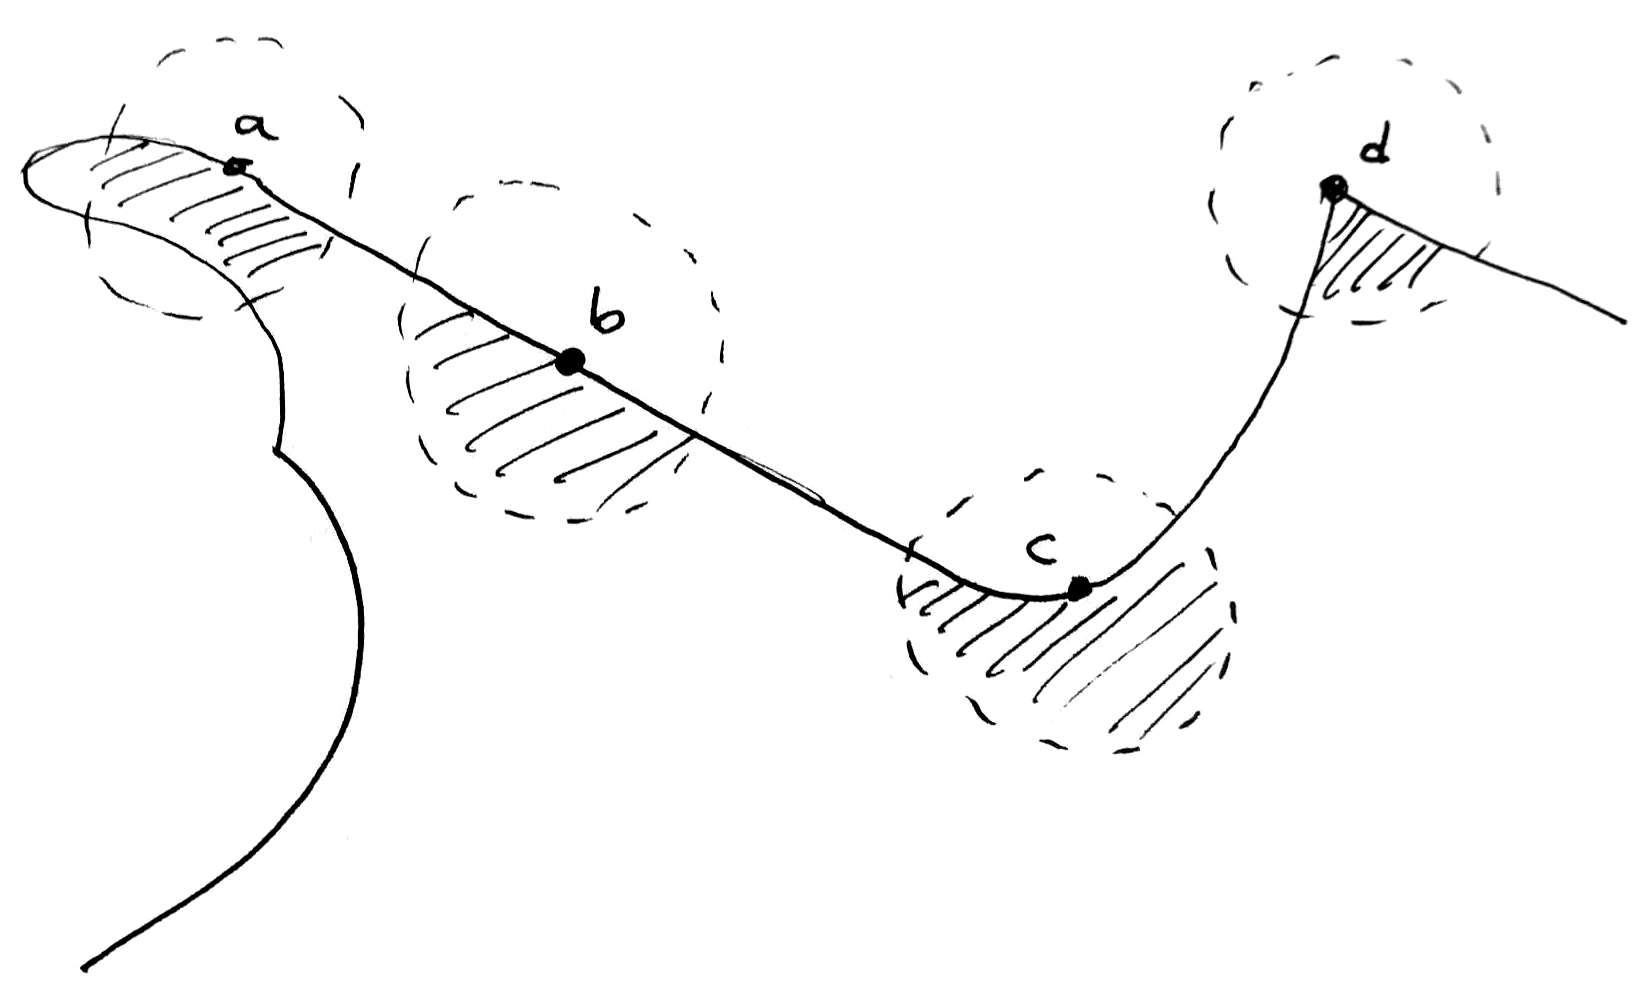
\includegraphics[width=0.6\linewidth]{f/figure1.png}
	\caption{
		Illustration of the rank transform
		when~$\kappa=\frac1{\pi r^2}\mathbf{1}_{B(r)}$ is the
		indicator function of a disk and~$\sigma$ is a Heaviside
		function.
		%
		This figure shows a level line of an image and four points
		on it.  In each case, the value of the rank transform is the
		proportion of the area of the disk that is intersected by
		the upper level set of the image (shaded regions around each
		point).
		%
		At point~$b$, the level line is locally straight and the
		value of the rank transform is~$1/2$.  At point~$c$, the
		level set is concave and the rank transform is~$>1/2$.  At
		point~$d$ the rank transform is~$\theta/{2\pi}$
		where~$\theta$ is the angle between two segments of the
		level line around that point.
	}
	\label{fig:figure1}
\end{figure}

TODO: write intuitive definition in terms of area percent of the support
of~$\kappa$ is covered by the level sets of~$u$.  Add a FIGURE for this.

Definition~\ref{def:krt} can be adapted to the case of discrete
images~$u:\mathbf{Z}^2\to\mathbf{R}$ by rewriting it in the measure
space~$\mathbf{Z}^2$ instead of~$\mathbf{R}^2$.  This results in the
following definition:

\begin{definition}\label{def:dkrt}
Let~$u:\mathbf{Z}^2\to\mathbf{R}$ be a bounded image,
$\kappa:\mathbf{Z}^2\to\mathbf{R}$ be a summable function
and~$\sigma:\mathbf{R}\to\mathbf{R}$ a non-decreasing function.
The~\emph{discrete kernel rank transform of~$u$ with kernel~$\kappa$
and comparison function~$\sigma$} is the
image~$\textsc{krt}_{\kappa,\,\sigma}(u):\mathbf{Z}^2\to\mathbf{R}$
defined by \begin{equation}\label{eq:rtdef}
%R_{\kappa}(u)(x) = \int\kappa(x-y)\mathbf{1}_{\left[u < u(x)\right]}(y)\mathrm{d}y
%R_{\kappa,\,\sigma}(u)(x) = \sum_{y\in\mathbf{Z}^2}\kappa(y-x)\sigma\parens{u(x)-u(y)}
	\textsc{krt}_{\kappa,\,\sigma}(u)(x) = \sum_{y\in\mathbf{Z}^2}\kappa(x-y)\sigma\parens{u(x)-u(y)}
\end{equation}
%by construction,~$R_\kappa(u)$ is an image that takes values in the
%interval~$[0,1]$.
\end{definition}

The original definition of the rank transform given by
equation~(\ref{eq:rt}) is a particular case of this definition by taking
the following~$\kappa$ and~$\sigma$:
\[
	\kappa=\mathbf{1}_{N_d(0)}
	\qquad
	\qquad
	\sigma(t)=\begin{cases}0&t\le0\\1&t>0\end{cases}
\]
where~$N_d(0)$ is a symmetric~$d\times d$ neighborhood of the origin.

The original definition is useful and practical, but it has a slightly
disturbing asymmetry in its comparison function~$\sigma$.  While this
asymmetry as a minor impact in practical cases, it is nonetheless very
visible when computing the rank transform of synthetic images, or images
with saturated regions.  Indeed, in locally constant parts of the image, the
rank transform is zero.  Notice that this problem cannot be solved by
changing the~$<$ condition in the definition to~$\le$, in that case constant
regions would get the value~$d^2-1$.
%(TODO: maybe point to some figure).

Henceforth, when we talk about the classical rank transform we will mean the
version with the balanced Heaviside~$H$ defined above.  With this choice,
constant patches get an intermediate value of~$1/2$.



\subsection{Equivalent definitions}

%We can rewrite the definition above in terms of the heaviside step
%function~$H(x)=\mathbf{1}_{[0,+\infty[}(x)$:
%\begin{equation}
%R_\kappa(u)(x)=
%\int
%\kappa(x-y)
%H\left(u\left(x\right)-u\left(y\right)\right)
%\mathrm{d} y
%\end{equation}

Definition~\ref{def:krt} looks formally similar to a convolution.

In fact, it can be written as a convolution in~$(x,u)$ space.
The epigraph of an image~$u:\mathbf{R}^2\to\mathbf{R}$ is the
function~$U:\mathbf{R}^2\times\mathbf{R}\to\mathbf{R}$ defined by
\[
	U(x,t) = \begin{cases}
		0 & \textrm{if $\ t< u(x)$} \\
		1 & \textrm{if $\ t\ge u(x)$}
	\end{cases}
\]
Then we define the ``kernel''
\[
	K(x,t) = \kappa(x)\delta(t)
\]
And now the convolution of~$U$ and~$K$ is
\[
	(U*K)(\xi,\tau)
	=
	\int
	\int U\left(y,t\right)K\left(\xi-y,\tau-t\right)
		\mathrm{d} y
		\mathrm{d} t
\]
\[
	\quad
	=\int
	U(y,\tau)
	\kappa(\xi - y)
		\mathrm{d} y
\]
\[
	\quad
	=\int\kappa(\xi-y)H(\tau - u(y))
		\mathrm{d} y
\]
Thus
\begin{equation}\label{eq:convolution1}
	\textsc{krt}_\kappa(u)(x)=(U*K)(x,u(x))
\end{equation}

Example in dimension 1 and k=interval.  Add THE FIGURE

Example in dimension 2 (image)

\begin{proposition}
Let~$U(x,t)$ be the epigraph of~$u$ as above, and let~$T=K*S$,
where~$K(x,t)=\kappa(x)\delta(t)$ and~$S(x,t)=\delta(x)\sigma'(t)$.  Then
\[
	\textsc{krt}_{\kappa,\sigma}(u)(x) = (U*T)(x,u(x))
\]
\end{proposition}
In other words, the~$\textsc{krt}$ is obtained by
linear-filtering the epigraph of~$u$ and evaluating the resulting filtered
3D image along the graph of~$u$.

TODO: check whether we can write~$T(x,t)=\kappa(x)\sigma'(t)$.

TODO: write the proof of the proposition above

\subsection{Formal properties}

%When~$\sigma$ is the Heaviside step function, we write simply~$R_\kappa$.

\begin{proposition}[structural properties of~$\textsc{krt}_{\kappa,\sigma}$]
	The kernel rank transform operator has the following properties:
	\begin{enumerate}
		\item[\bf P1] If~$u$ is a constant image,
			then~$\textsc{krt}_{\kappa,\sigma}(u)=\sigma(0)\int\kappa$.
		\item[\bf P2] Scaling and shifting of~$\sigma$:
			$\textsc{krt}_{\kappa,\,a\sigma+b}=a\,\textsc{krt}_{\kappa,\sigma}+b\int\kappa$.
		\item[\bf P3] Symmetry with respect to inversion: if~$\sigma$
			is an odd function
			then~$\textsc{krt}_{\kappa,\sigma}(-u)=-\textsc{krt}_{\kappa,\sigma}(u)$.
		\item[\bf P4] If~$\kappa$ is symmetric and~$\sigma$ is
			anti-symmetric ($\sigma(-t)+\sigma(t)=\sigma(0)$),
			and~$u$ is an affine function
			then~$\textsc{krt}_{\kappa,\sigma}=\sigma(0)\int\kappa$.
		\item[\bf P5] If~$\varphi(x)=Ax+b$ is an affine map
			of~$\mathbf{R}^2$
			then\\
			$\displaystyle
			\textsc{krt}_{\kappa,\sigma}\left(u\circ\varphi\right) =
			%\textsc{krt}_{\frac1{|A|}\kappa\circ A^{-1},\sigma}\left(u\right)\circ\varphi$.
			\textsc{krt}_{\tilde\kappa,\sigma}\left(u\right)\circ\varphi$,
			where~$\tilde\kappa=\frac1{|A|}\kappa\circ A^{-1}$.
%		\item[\bf P5] If~$\tau$ is a translation
%			of~$\mathbf{R}^2$
%			then~$R_{\kappa,\sigma}\left(u\circ \tau\right) =
%			\left(R_{\kappa,\sigma} u\right)\circ\tau$.
%		\item[\bf P6] If~$\rho$ is a rotation
%			of~$\mathbf{R}^2$
%			then~$R_{\kappa,\sigma}\left(u\circ\rho\right) =
%			\left(R_{\kappa\circ\rho,\sigma} u\right)\circ\rho$.
		\item[\bf P6] The value of~$\textsc{krt}_{\kappa,\sigma}(u)(x)$
			only depends on the values of~$u$ on the
			set~$\left\{x+y\ |\ y\in\mathrm{supp}(\kappa)\right\}$.
		\item[\bf P7] Quasi-invariance under affine contrast changes:
		$\textsc{krt}_{\kappa,\sigma}(\alpha u+\beta)(x)
		=
		\textsc{krt}_{\kappa,\tilde\sigma}(u)(x)
		$
		with~$\tilde\sigma(t)=\sigma(\alpha t)$.
	\end{enumerate}
\end{proposition}

Properties P1 and P4 also hold locally with respect to~$u$, where locality is
defined by the support of~$\kappa$.

Property~P2 says that the scaling of the function~$\sigma$ is an essentially
arbitrary convention: for example, we can replace the Heaviside with a sign
function and the results vary
accordingly:~$\textsc{krt}_{\kappa,\mathrm{sgn}}=2\,\textsc{krt}_{\kappa,H}-\int\kappa$.
For normalized and symmetric kernels, the result will then take values in
the range~$[-1,1]$, being~$0$ on flat zones or zones where the level lines
are straight.

Property~P5 says two things.  First, that the transform is covariant with
translations~$b$ (this is the particular case when~$A$ is the identity
matrix).  Second, that it is also covariant with linear maps~$A$, but the
kernel~$\kappa$ must be rescaled accordingly.  This property is an immediate
consequence of the change of variables formula.

The localization property~P6 becomes clear when one notices that the
integral defining $\textsc{krt}_{\kappa,\sigma}(u)(x)$ can be reduced to an
integral over the support of~$\kappa$ centered around~$x$.

\begin{proposition}
	When~$\sigma$ is the balanced Heaviside step function (eq.\ref{eq:heaviside}),
	the kernel rank
	transform has these further properties:
	\begin{enumerate}
		\item[\bf H1] Invariance under arbitrary contrast changes: for
			any increasing injective function~$g$, we
			have~$\textsc{krt}_{\kappa,H}(g\circ
			u)=\textsc{krt}_{\kappa,H}(u)$.
		\item[\bf H2] If~$x$ is the site of the strict global
			maximum of~$u$,
			then~$\textsc{krt}_{\kappa,H}(u)(x)=\int\kappa$.  This is also
			true if~$x$ is a strict local maximum on a
			neighborhood defined by the support of~$\kappa$.
		\item[\bf H3] If~$x$ is the site of the strict global
			minimum of~$u$, then~$\textsc{krt}_{\kappa,H}(u)(x)=0$.  This
			is also true if~$x$ is a strict local minimum on a
			neighborhood defined by the support of~$\kappa$.
	\end{enumerate}
\end{proposition}

Note: all the properties above except P5 are valid for both the continuous
and the discrete versions of the KRT (definitions~\ref{def:krt}
and~\ref{def:dkrt}).  Property~P5 makes sense only in the continuous case.


%Fundamental property: invariance under arbitrary contrast changes (without
%change inversion).~$R_k(g\circ u)=R_k(u)$, for any increasing injective
%function~$g$
%
%Symmetry with respect to inversion:~$R_k(-u)=1-R_k(u)$
%
%If~$x$ is the site of the global maximum of~$u$, then~$R_\kappa(u)(x)=1$.
%This is also true if~$x$ is a local maximum on a neighborhood defined by the
%support of~$\kappa$.
%
%Correspondingly, if~$x$ is the site of the global minimum of~$u$,
%then~$R_\kappa(u)(x)=0$.
%
%If the level lines of~$u$ are straight lines with the same orientation (for
%example, when~$u$ is affine), and~$\kappa$ is symmetric,
%then~$R_\kappa(u)=\frac12$.


\subsection{Continuity and differentiability}

The experiments on figures~\ref{fig:machup} and~\ref{fig:machdown} show that
the kernel rank transform (without step) is a~\emph{discontinuous}
transformation of the original gray-levels.  The figure shows that two
images that are nearly identical have very different rank transforms.  This
is a general phenomenon: contrast invariance is a non-differentiable
property.  In other words, any contrast-invariant operator will be likewise
discontinuous:

\begin{definition}[contrast-invariant filter]
	Let~$T$ be an operator that transforms gray-level images into images
	of the same type.  We say that it is~\emph{contrast-invariant} if
	for any
	monotonic function~$g:\mathbf{R}\to\mathbf{R}$ and for any image~$I$
	we have~$T(g\circ I)=T(I)$.
\end{definition}

\begin{proposition}
	Any continuous and contrast-invariant image filter is trivial.
	%(its result does not depend on the input image).
\end{proposition}
\begin{proof}
	Let~$T$ be a contrast-invariant filter that is continuous (with
	respect to some norm, for example~$L^2$ or~$L^\infty$).
	Now, fix an image~$I$ and consider the
	path~$\lambda\mapsto \lambda I$ in the space of images.  By
	homogeneity of the norm, this path
	is a continuous curve that joins the image~$I$ to the image~$0$.
	Since the filter is continuous,~$\displaystyle\lim_{\lambda\to
	0+}T(\lambda I)=T(0)$.
	Since the filter is contrast-invariant,~$T(\lambda I)=T(I)$
	for all~$\lambda>0$.
	Thus~$T(I)=T(0)$ and the filter is trivial.
\end{proof}

\begin{corollary}
	Any non-trivial contrast-invariant filter is discontinuous.
\end{corollary}

This proposition showcases an important compromise between the two cases of
the kernel rank transform.
The kernel rank transform with a smooth step~$\sigma$, as defined on
equation~\ref{eq:rtdef} is continuous with respect to~$u$ by continuity
under the integral sign.  Thus, it cannot be contrast-invariant.  The
function~$t\mapsto\sigma(t)$ controls precisely how much contrast-invariance
is lost: a gray-levels~$t_1$ is considered brighter than a gray-level~$t_2$
only when~$\sigma(t_1-t_2)$ is close to~$1$.

For a smooth~$\sigma$ we can explicitly compute the variation of
\begin{equation}
	\textsc{krt}_{\kappa,\,\sigma}(u)(x) = \int\kappa(y-x)\sigma\parens{u(x)-u(y)}\mathrm{d}y
\end{equation}
along the direction~$v$ as
\begin{equation}\label{eq:dkrt}
	\frac{\delta \textsc{krt}_{\kappa,\,\sigma}(u)(x)}{\delta v}
	= \int\kappa(y-x)\sigma'\parens{u(x)-u(y)}\parens{v(x)-v(y)}\mathrm{d}y
\end{equation}
where
\begin{equation}
	\frac{\delta \textsc{krt}_{\kappa,\,\sigma}(u)(x)}{\delta v}
	=
	\lim_{\varepsilon\to0}
	\frac{\textsc{krt}_{\kappa,\,\sigma}(u+\varepsilon v)(x)
	-\textsc{krt}_{\kappa,\,\sigma}(u)(x)}{\varepsilon}.
\end{equation}
This derivative measures how the kernel rank transform of~$u$ changes
when the image~$u$ is slightly deformed on the direction of an image~$v$.
This shows that the kernel rank transform is a smooth operation through
which information can be backpropagated.

Formula~\ref{eq:dkrt} can be interpreted easily when~$v$ is a small Gaussian
centered around a point~$z$.  In that case, $\frac{\delta
\textsc{krt}_{\kappa,\,\sigma}(u)(x)}{\delta v}$ measures how
does~$\textsc{krt}_{\kappa\,\sigma}u(x)$ changes when~$u(z)$ changes.
We distinguish two cases, depending on whether~$z$ is close to~$x$ or not.
When~$z$ is very far from~$x$, the term~$v(x)-v(y)$ is a Gaussian centered
around~$z$, and the term~$\kappa(y-x)$ is centered around~$x$, thus their
product is very close to 0.  This means that the KRT is a local operator,
with a receptive field modulated by the function~$\kappa$.  When~$z=x$, the
term~$v(x)-v(y)$ is of the form~$a(1-e^{-b(y-x)^2})$, which vanishes
at~$y=x$, and when multiplied by~$\kappa(y-x)$ gives a ring-shaped ``receptive
field'' around~$x$.  The receptive field is further reduced after
multiplication by~$\sigma'\parens{u(x)-u(y)}$, which is a fuzzy region
around the level line of~$u$ through~$x$.

TODO: add figure with said receptive field (maybe in 1d and for a discrete
image also? the case of the discrete image is easy: just compute the
directional derivative when changing a single pixel)

TODO: comment what happens when~$\sigma$ is a heaviside (the derivative
cannot be computed manually)

TODO: some further comments about locality around the level line.


\subsection{Normalization and Visualization}

Typical ranges: $[1,N^2]$, $[0,1]$, $[-1,1]$

Visualization: gray-scale, signed
%(point to a later section where the link to curvature is explained)

\subsection{Infinitesimal generator}

In this section we study the effect of the kernel rank
transform~$\textsc{krt}_{G_h,\sigma}$ for Gaussian kernels
$G_h(x)=\frac1{2\pi h^2}\exp\frac{-\|x\|^2}{2h^2}$ as~$h\to 0$.
We will see that there are two different behaviours depending on the
regularity of~$\sigma$ at~$0$.  If~$\sigma$ is smooth around 0, then the
local effect of the KRT is equivalent to a convolution by~$G_h$, whose infinitesimal
generator is the Laplacian operator:
\begin{equation}\label{eq:localsmooth}
	\textsc{krt}_{G_h,\sigma}(u)(x)=\sigma(0)+\sigma'(0)\Delta u(x)\frac{h^2}2+O(h^3)
\end{equation}
On the other hand, if~$\sigma$ is discontinuous around 0, like
the centered Heaviside function~$\sigma=H$, then the generator is the curvature
operator
\begin{equation}\label{eq:localheaviside}
	\textsc{krt}_{G_h,H}(u)(x)=\frac12+\frac1{4\sqrt{2\pi}}\mathrm{curv}(u)(x)h+O(h^2)
\end{equation}
where~$\mathrm{curv}(u)(x)=\mathrm{div}\left(\frac{\nabla u}{\|\nabla
u\|}\right)$.  
Propositions~\ref{thm:contistep} and~\ref{thm:krtheaviside}
below give full statements and proofs of these two results, where the kernel
is not necessarily Gaussian.




% Start with the case of a disk
Case of a square kernel and a parabolic level line\\
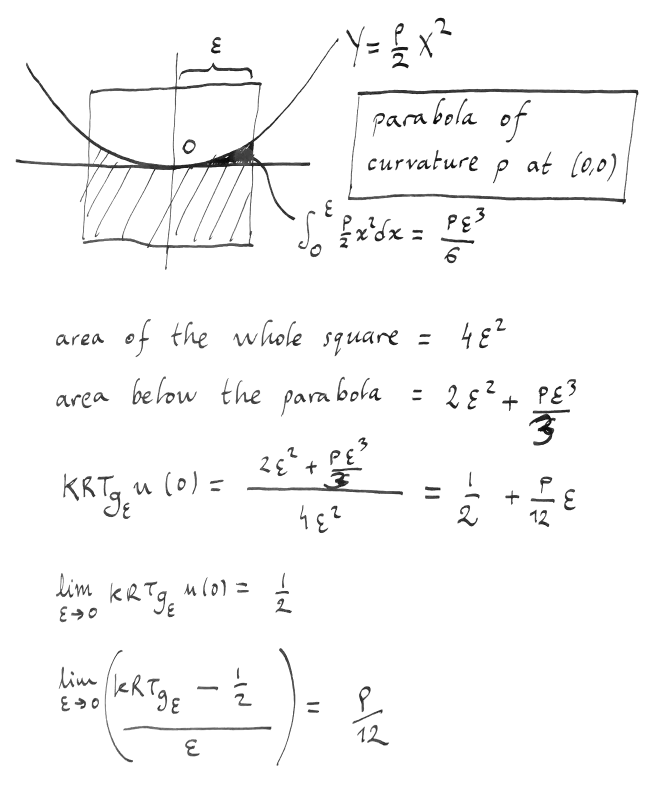
\includegraphics[width=0.6\linewidth]{f/pcurv.png}




% check the term ``germ'' below
Recall the following result: the ``germ'' of a blur is the laplacian.  Below
we will see that the ``germ'' of the krt is the curvature of the level
lines.

\begin{definition}
	A~\emph{laplacian-consistent kernel} is a
	function~$g:\mathbf{R}^2\to\mathbf{R}$ with the following
	properties:~$\int g=1$, $\int g(x)x\mathrm{d} x=
	\left(\begin{smallmatrix}0\\0\end{smallmatrix}\right) $,
	$\int g(x)x\otimes x\mathrm{d}
	x=\left(\begin{smallmatrix}1&0\\0&1\end{smallmatrix}\right)$ and
	$\int \left|g(x)\right|\left\|x\right\|^3\mathrm{d} x<+\infty$.
\end{definition}

\begin{remark}
	The condition of laplacian consistency can be written using the following
	notation for the momnets.  If we define the~$p$ moment of~$g$
	as~$M_p(g)=\int g(x)x^{\otimes p}dx$ (a tensor of order~$p$).  Then~$g$ is
	laplacian-consistent when~$M_0(g)=1$, $M_1(g)=0$, $M_2(g)=I_2$
	and~$M_3(g)<+\infty$.
\end{remark}

Notice that if~$g$ is a laplacian-consistent kernel, then each function of
the family
\[
	g_h(x)=\frac1{h^2}g\left(\frac{x}{h}\right)
\]
is as well, for~$h>0$.  Let us recall first the following classical result (cf. 
Alvarez, Morel, Florack )

\begin{proposition}[Laplacian approximation]
	Let~$g$ be a laplacian-consistent kernel.
	Then~$g_h-\delta$ gives a good approximation of the
	Laplacian when~$h\to 0$.  More precisely, if~$u\in C^3(\mathbf{R}^2)$
	is bounded and all its derivatives up to order 3 are bounded,
	then
	\[
		%\lim_{h\to 0}
		%\frac{g_h*u(x)-u(x)}{h^2}=\frac{\rho^2}{2}\Delta u(x).
		g_h*u(x)=u(x)+\Delta u(x) \frac{h^2}{2} + O(h^3).
	\]
\end{proposition}
\begin{proof}
	Write down~$g_h*u(x)$:
	\[
		g_h*u(x)
		=\int \frac1{h^2}g(t/h)u(x-t)d t
		=\int g(y)u(x-hy)d y
	\]
	and develop~$u(x-hy)$ by
	Taylor
	\[
		g_h*u(x)
		=
		\int
		\left(
		u(x)
		-hDu(x)\cdot y
		+\frac{h^2}2D^2u(x)(y,y)
		+O(h^3\|y\|^3)
		\right)
		g(y)
		dy
	\]
	now, since~$x$ is fixed, the first three integrals can be computed thanks
	to the first three properties of laplacian consistency, to
	obtain~$u(x)+0+\frac{h^2}2\Delta u(x)$.  The remaining term can be
	written as~$O(h^3)$ thanks to the hypotheses $\int|g(y)|\|y^3\|dy<+\infty$
	and~$|D^3u|<M$.
\end{proof}

\begin{lemma}(local effect of KRT with polynomial step)
	\label{lem:polystep}
	Let~$g$ be a kernel with finite moments up to order~$p$, $M_p(g)=\int
	g(x)x^{\otimes p}dx$ and~$u\in C^2$ with bounded second derivatives.  Then
\[
	\textsc{krt}_{g_h,s^p}(u)(x)=h^pM_p(g)\left(\nabla u(x)\right)^p  +
	O(h^{p+1})
\]
where~$M_p(g)(v)^p=M_p(g)(v,\cdots,v)$ means the~$p$-dimensional tensor~$M_p(g)$ applied
to~$p$ copies of the vector~$v$.
\end{lemma}

\begin{proof}
	First, notice that
	\[
		\int g(t)(v\cdot t)^pdt=M_p(g)(v)^p
	\]
	as can be readily checked using Einstein notation.

	Now,
	\begin{align*}
		\textsc{krt}_{g_h,s^p}(u)(x)
		&=\int g_h(x-y)\big(u(x)-u(y)\big)^pdx\\
		&=\int g(t)\big(u(x)-u(x-ht)\big)^pdt\\
	\end{align*}
	and, by Taylor expansion of~$u$ we have
	$u(x)-u(x-ht)=h\nabla u(x)\cdot t + O(h^2)$, thus
	\begin{align*}
		\textsc{krt}_{g_h,s^p}(u)(x)
		&=\int g(t)\big(h\nabla u(x)\cdot t+O(h^2)\big)^pdt\\
		&=\int g(t)\big(h^p(\nabla u(x)\cdot t)^p+O(h^{p+1})\big)dt\\
		&=h^p\int g(t)(\nabla u(x)\cdot t)^pdt + O(h^{p+1})\\
		&=h^pM_p(g)(\nabla u(x))^p+O(h^{p+1})
	\end{align*}
\end{proof}


The following two propositions characterize the local effect of applying the
KRT with kernels~$g_h$.

% NOTE: normalize the meaning of h in the propositions below (proposition 7
% uses a different scaling, not according to that after the definition of
% laplacina consistency.

\begin{theorem}[Local effect of KRT with continuous step]
	\label{thm:contistep}
	Let~$g$ be a laplacian-consistent kernel, and~$u$ be~$C^3$ with bounded
	derivatives up to order~$3$.
	Let~$\sigma:\mathbf{R}\to\mathbf{R}$ be a~$C^2$ function with bounded
	derivatives up to order~$3$.
	Then
	\[
		\textsc{krt}_{g_h,\sigma}(u)(x) = \sigma(0)
		+
		\frac{
			\sigma'(0)\Delta u(x)
			+
			\sigma''(0)\left\|\nabla u(x)\right\|^2
		}2
		h^2
		+O(h^3)
	\]
\end{theorem}
\begin{proof}
	The result is obtained by linearity of~$\textsc{krt}_{g_h,\sigma}(u)$ with
	respect to~$\sigma$ and the Taylor expansion of~$\sigma$:
	\[
		\sigma(r)=\sigma(0)+\sigma'(0)r+\frac{\sigma''(0)}2r^2+\frac{\sigma'''(\xi)}{3!}r^3
	\]
	for some~$\xi\in[0,r]$, and the last term can be bounded by a constant
	by the hypotheses.
%	By the hypotheses on~$s$ we can write
%	\[s(r)=s(0)+s'(0)r+\frac12s''(\xi)r^2\]
%	for some~$\xi\in[0,r]$.  Replacing this into the definition of the Kernel
%	Rank Transform:
%	\[
%		\textsc{krt}_{g_h,s}(u)(x) = \int g_h(x-y)s(u(x)-u(y))dy
%	\]
%	\[
%		\textsc{krt}_{g_h,s}(u)(x) =
%		\int
%		g_h(x-y)
%		\left(
%		s(0)
%		+(u(x)-u(y))s'(0)
%		+\frac{s''(\xi)}2(u(x)-u(y))^2
%		\right)
%		dy
%	\]
%	the first term is equal to~$s(0)$; by the previous result, the second term
%	is equal to~$\frac{s'(0)\rho^2}2\Delta u(x)h^2+O(h^3)$.  It remains to
%	prove that~$\int g_h(x-y)(u(x)-u(y))^2dy\in O(h^3)$.
%
%	By linear change of variable, we write this integral as
%	\[
%		\int g(t)(u(x)-u(x-th))^2dt
%	\]
%
\end{proof}





\clearpage
\begin{lemma}\label{lem:curv1}
	Let~$u:\mathbf{R}^2\to\mathbf{R}$ such that the level line~$u=u(0,0)$ is a
	function of equation~$Y=c(X)$, smooth in a neighborhood of the origin,
	with~$c(0)=c'(0)=0$.
	Let~$g:\mathbf{R}^2\to\mathbf{R}$ be a symmetric, normalized,
	eventually decreasing kernel such that~$\rho=\int_{-\infty}^\infty
	x^2g(x,0)\mathrm{d} x<+\infty$, $\int_{-\infty}^\infty x^3g(x,0)dx<+\infty$ and~$\int_{-\infty}^\infty x^4g_y(x,0)\mathrm{d}
	x<+\infty$.  Then, if we
	denote~$g_h(x,y)=\frac1{h^2}g(x/h,y/h)$,
	\[
		\textsc{krt}_{g_h,H}(u)(0)=\frac12+\frac{c''(0)}2\rho h+O(h^2)
	\]
\end{lemma}

\begin{proof}
	Let us write the definition of~$\textsc{krt}_{g_h,H}(u)(0)$:
	\[
		\textsc{krt}_{g_h,H}(u)(0)=
		\int_{-\infty}^\infty\int_{-\infty}^{c(x)}
		g_h(x,y)\ %
		\mathrm{d}y
		\mathrm{d}x
	\]
	\[
		=
		\int_{-\infty}^\infty\int_{-\infty}^{c(x)}
		\frac1{h^2}g\left(\frac{x}{h},\frac{y}{h}\right)\ %
		\mathrm{d}y
		\mathrm{d}x
	\]
	\[
		=
		\int_{-\infty}^\infty\int_{-\infty}^{c\left(hx\right)/h}
		g\left(x,y\right)\ %
		\mathrm{d}y
		\mathrm{d}x
	\]
	Now, this is a function of~$h$, let us call it~$f(h)$, that we can
	develop by Taylor:~$f(h)=f(0)+f'(0)h+\frac12f''(0)h^2+\cdots$.
	Notice that~$c(hx)/h$ is well-defined for~$h=0$ since
	$c(hx)/h=c''(0)hx^2/2+O(h^2)$.
	Now we have that~$f(0)=\frac12$ by symmetry of~$g$.  Now
	\[
		f'(h)=
		\int_{-\infty}^\infty \frac{d}{d h}\left(\frac{c(hx)}h\right)
		\left[\vphantom{\int}g(x,y)\right]_{-\infty}^{c(hx)/h}
		\ \mathrm{d}x
		=
		\int_{-\infty}^\infty \left(\frac{x^2c''(0)}2+O(h)\right)
		g\left(x,\frac{c\left(hx\right)}h\right)
		\ \mathrm{d}x
	\]
	thus
	\[
		f'(0)=\frac{c''(0)\rho}2
		%\int_{-\infty}^\infty \frac{\kappa x^2}2
		%g(x,0)\ \mathrm{d}x
		%=\frac{\kappa\sigma^2}2.
	\]
	By further differentiation of~$f'(h)$ we obtain
	\[
		f''(0)=
		\frac{c'''(0)}6\int_{-\infty}^\infty x^3g(x,0)dx
		+
		\frac{c''(0)^2}4\int_{-\infty}^\infty x^4g_y(x,0)dx
	\]
	which is finite by the hypotheses.
\end{proof}


\clearpage
\begin{theorem}[behavior of the KRT with Heaviside step]
	\label{thm:krtheaviside}
	Let~$u:\mathbf{R}^2\to\mathbf{R}$ and~$x\in\mathbf{R}^2$ such that
	the level line~$[u=u(x)]$ is a smooth curve on a neighborhood
	of~$x$.  Let~$g:\mathbf{R}^2\to\mathbf{R}$ be a radial,
	normalized kernel with
	finite moments.  Then, if we
	denote~$g_h(x)=\frac{1}{h^2}g(x/h)$,
	\[
		\textsc{krt}_{g_h,H}(u)(x)=\frac12+\frac\gamma{4\pi}\mathrm{curv}(u)(x) h+O(h^2)
	\]
	where~$\gamma=\int_{\mathbf{R}^2}g(x)\|x\|dx$ and
	$\mathrm{curv}(u)(x)=\mathrm{div}\left(\frac{\nabla
	u}{\left\|\nabla u\right\|}\right)$.
\end{theorem}

\begin{proof}
	This is a consequence of the previous proposition.
	There are several localization steps that allow us to reduce this theorem
	to the previous result.  The main problem is that the level line
	through~$u(x)$ need not be the graph of a function, as required.

	First, thanks to property P5, the domain can be translated and rotated so
	that~$x=(0,0)$ and the level line through that point is horizontal.  This
	transformation does not change the curvature of the level line.

	By the hypotheses, we can assume that the level curve
	is of the form~$t\mapsto(t,c(t))$ inside~$B_R(0)$ for some~$R>0$.
	So, without loss of generality we can assume that~$c(0)=0$ and~$c'(0)=0$.
	Notice that~$c''(0)=\mathrm{curv}(u)(0)$ is the curvature of the curve at
	the point~$(0,0)$.

	To apply the previous proposition, we will extend the function~$u$ outside
	of~$B_R(0)$ so that the level line is the graph of a
	function~$\mathbf{R}\to\mathbf{R}$.  For example, we can set~$\tilde
	u(y)=\begin{cases}u(y)&\textrm{if }\|y\|\le
	R\\u\left(\frac{Ry}{\|y\|}\right)&\textrm{otherwise}\end{cases}$.
	We define as well the finite-support kernel~$g_h^R=\mathbf{1}_{B_R(0)}g_h$.

	We will now show a chain of approximations
	\[
	 \textsc{krt}_{g_h,H}(u)(x)
	 \approx
	 \textsc{krt}_{g^R_h,H}(u)(x)
	 =
	 \textsc{krt}_{g^R_h,H}(\tilde u)(x)
	 \approx
	 \textsc{krt}_{g_h,H}(\tilde u)(x)
	\]
	The middle equality is a direct consequence of localization property~P6.
	We will prove that the error of the two remaining approximations is
	bounded by~$\frac{h^2 m_2(g)}{R^2}$,
	where~$m_2(g)$ is the second moment of~$|g|$ which is finite by
	hypothesis.

	Indeed, the
	error $\left|\textsc{krt}_{g_h,H}(u)(x)-\textsc{krt}_{g_h^R,H}(u)(x)\right|$
	can be bounded.
	By the triangle inequality:
	\[
		\left|
		\int g_h(x-y)H(u(x)-u(y))dy
		-
		\int g_h^R(x-y)H(u(x)-u(y))dy
		\right|
		\le
		\int
		\left|
		g_h
		-g_h^R
		\right|
	\]
	This error term is the ``tail'' of~$g_h$ which can be controlled because
	\[
		\int
		\left|
		g_h
		-g_h^R
		\right|
		=
		\int_{|y|\ge R} \left|g_h\right|
		\le
		\int_{|y|\ge R} \left|g_h(y)\right|\frac{\|y\|^2}{R^2}dy
		=
		\int_{|z|\ge R/h} h^2\left|g(z)\right|\frac{\|z\|^2}{R^2}dz
		\le
		\frac{h^2m_2(g)}{R^2}.
	\]
	And the same argument proves that~$\left|\textsc{krt}_{g_h,H}(\tilde
	u)(x)-\textsc{krt}_{g_h^R,H}(\tilde u)(x)\right|\le\frac{h^2m_2(g)}{R^2}$.
	This means that the errors of each approximation are~$O(h^2)$.

	Now we can apply the previous proposition to the kernel~$g$ and
	function~$\tilde u$ at point~$x=0$.  Notice that~$\rho$, as defined in the
	previous proposition is equal to~$\frac{\gamma}{2\pi}$ since the kernel is
	radial (otherwise,~$\rho$ would depend on the angle of rotation).  Then, the
	proposition reads
	\[
		\textsc{krt}_{g_h,H}(\tilde
		u)(x)=\frac12+\frac{\gamma}{4\pi}\mathrm{curv}(u)(x)h + O(h^2)
	\]
	which, together with the approximation
	\(
		\textsc{krt}_{g_h,H}(u)=\textsc{krt}_{g_h,H}(\tilde u)+O(h^2)
	\)
	concludes the proof.
\end{proof}

The previous theorem % TODO add ref?
describes the local behavior of the KRT with Heaviside step.
It can be stated as ``the infinitessimal generator of the KRT is the
curvature operator~$\mathrm{div}\left(\frac{\nabla u}{\left\|\nabla
u\right\|}\right)$''.
This is analogous to theorem  % TODO add ref?
which can be stated as ``the infinitessimal generator of Gaussian blur is
the laplacian operator~$\Delta u$.''
These two results deal with the case where~$u$ is smooth, otherwise the
derivatives don't make sense.  In the case of the KRT with Heaviside step,
the result above has a stronger requirement than the level lines of~$u$ are
smooth (which will not be the case in general, even for $u\in C^\infty$).  The
next proposition describes the behaviour of the KRT with Heaviside step
at a critical point where the level lines meet at an angle or at a cusp.


\clearpage
\begin{theorem}[Heaviside KRT with an angle]
	Let~$u:\mathbf{R}^2\to\mathbf{R}$ and~$x\in\mathbf{R}^2$ such that
	the level line~$[u=u(x)]$ is a piecewise smooth curve with an
	angle~$\alpha$ at~$x$.
	Let~$g:\mathbf{R}^2\to\mathbf{R}$ be a radial,
	normalized kernel with
	finite moments.  Then, if we
	denote~$g_h(x)=\frac{1}{h^2}g(x/h)$,
	\[
		\textsc{krt}_{g_h,H}(u)(x)=\frac\alpha{2\pi}
		+
		\frac\gamma{4\pi}\left(\frac{\kappa_1+\kappa_2}2\right) h+O(h^2)
	\]
	where~$\gamma=\int_{\mathbf{R}^2}g(x)\|x\|dx$ and
	$k_1$ and~$k_2$ are the curvatures of the level line at each side of the
	angle (see Figure).
\end{theorem}

Observation: the previous theorem is not completely general, as level lines
may have more complex behavior (for example, at a saddle point of~$u$ the
level lines will have an intersection).  This result can be generalized to
these situations.


\subsection{Iterated filtering}

The kernel rank transform $\textsc{krt}_\sigma$ is an operator that transforms images into images of the same size.
What happens when we compute iterates of this operator?   Is it idempotent?  Is it a semigroup?  Do the iterates explose? (unlikely since they are always images with values on the unit interval).

Some experimental observations with a Gaussian kernel of size
6:

The operator is not idempotent (show experiments with a synthetic and a small real image).

The operator is not a semigroup on the parameter $\sigma$.  We built a list
of a few hundred images $\textsc{krt}_\sigma(u)$ with finely varying
$\sigma$, and we compared them to $\textsc{krt}(\textsc{krt}_6(u))$.  They are all very different, the closet one being about $\sigma=4.4$.

The iterates $\textsc{krt}^n(u)$ seem to converge to a fixed point.  The
fixed point does not look like any $\textsc{krt}_\sigma(u)$, the closest one being for~$\sigma=5.4$.

Apparently, we can define a limit operator~$\textsc{krt}^\infty_\sigma$ by
\[
	\textsc{krt}^\infty_\sigma(u) := \lim_{n\to\infty}\textsc{krt}^n_\sigma(u)
\]
We do not know whether these limit operators are the kernel rank transdform
for a different kernel.   If that was the case, the krt of that kernel
would be idempotent.

\subsection{Discretization artifacts}

some experiments with krt in a discrete setting using a heaviside step.
We observe that certain behaviours of the continuous case are not directly
inherited in the discrete case.

for~$u(x,y)=px+qy$ the level lines are straight lines.  Thus the krt is
constant equal to~$1/2$.  This behaviour is observed exactly in the discrete
case.  It can be seen also from the definition of the discrete krt (by
symmetry of the kernel).

if~$u$ is a distance function~$u(x)=\|x\|$ then its level lines are circles
of curvature~$1/\|x\|$.  for a kernel~$g_h$ with~$h\to 0$, the krt of this
function goes to~$1/2+1/(2\|x\|)$.  In the discrete case, the observed
behaviour is very different, especially for a kernel of small support.  Far
from the origin, most of the transformed image is equal to $1/2$, and the
other, higher values are concentrated at straight lines at 45 degrees, etc.

\subsection{Statistical properties}

If~$\mathcal{W}$ is a white gaussian noise image, then its KRT is a uniform
noise image.  The important property is the independence of pixels, the
initial distribution is not really important.  In the discrete setting, let
\[
	X_0,X_1,\ldots,X_n
\]
be identically distributed independent variables (+ additional hypotheses).
Define a variable
\[
	Y = \sum k_i H(X_i-X_0)
\]
where~$k_i$ are a set of real numbers whose sum is 1 (+ additional
hypotheses).  Then~$Y$ is close to a discrete uniform distribution
in~$[0,1]$.  This closeness will be formalized below as a limit.

Thus, the KRT transforms white noise into uniform noise.  There is a
tradeoff, however: whiteness is transformed into uniformity, but the
whiteness is lost.

Experimental observations: the KRT of white noise is negativelly correlated
with a profile that is minus the symmetrized kernel + some smaller
correction terms [this must be formalized somehow].

\bigskip

Some explicit computations.

Let~$\{X_p\}_p$ be the set of pixel values of an image.  Assume that the
pixels are independent variables following a continuous law, so that

$$
P(X_p=X_q)=0
\qquad
P(X_p<X_q)=\frac12
\qquad
P(X_p>X_q)=\frac12
$$

Let us start with a uniform kernel, defined by a neighborhood~$\mathcal{N}$
(which by convention does not contain the center 0).
Thus the~$KRT$ at a point~$p$ is a random variable, function of all the
variables~$X_i$ for all the pixels:

\[
	K_p = \sum_{i\in\mathcal{N}} \kappa_i H(X_p - X_{p+i})
\]

We will compute the law of this random variable, its expectation, and the
covariance between two such variables~$K_p$ and~$K_q$.

The case~$\kappa_i=1$ can be treated by elementary considerations, where the
variable~$K_p$ is discrete uniform with values between~$0$ and~$N-1$,
where~$N$ is the size of the neighborhood.
The case for a general kernel~$\kappa$ is more subtle and will be dealt with
later.

The computations for the expectation and covariance can be done directly for
arbitrary kernel coefficients~$\kappa_i$.

Let us compute the expectation of~$K_p$
\[
	E(K_p) = \sum_{i\in\mathcal{N}} \kappa_i E(H(X_p - X_{p+i}))
\]
and now~$E(H(X_p-X_{p+i}))=P(X_p>X_{p+i})=\frac12$.

Now let~$p,q$ be different pixel positions, we want to compute the
covariance between~$K_p$ and~$K_q$.

\[
	\mathrm{cov}(K_A,K_B)
	=
	E(K_AK_B)-E(K_A)E(K_B)
\]

let us develop this expression:

\[
	\mathrm{cov}(K_A,K_B)
	=
	\sum_{i\in N}
	\sum_{j\in N}
	\kappa_i\kappa_j
	\left(
	E
	\left(
	H(X_A-X_{A+i})H(X_B-X_{B+j})
	\right)
	-\frac14
	\right)
\]

these expectations have 4 possible values~$\frac16,\frac14,\frac13,\frac12$
depending on the relative positions of the 4 points, which may or may not
coincide.  This allows us to separate the whole sum according to the values of
these terms.

First, let us separate the cases~$B=A+i$ and~$A=B+j$:

\begin{align*}
	\mathrm{cov}(K_A,K_B)
	&=
	\sum_{i\in N,A+i\neq B}
	\sum_{j\in N,B+j\neq A}
	\kappa_i\kappa_j
	\left(
	E
	\left(
	H(X_A-X_{A+i})H(X_B-X_{B+j})
	\right)
	-\frac14
	\right)\\
	&+
	\sum_{j\in N}
	\kappa_{B-A}\kappa_j
	\left(
	E
	\left(
	H(X_A-X_B)H(X_B-X_{B+j})
	\right)
	-\frac14
	\right)\\
	&+
	\sum_{i\in N}
	\kappa_i\kappa_{A-B}
	\left(
	E
	\left(
	H(X_A-X_{A+i})H(X_B-X_A)
	\right)
	-\frac14
	\right)\\
\end{align*}

Now we separate the first term into the cases, depending on
whether~$A+i=B+j$ or otherwise (in which case the four pixels are different
and the expectation will be 0).


\begin{align*}
	\mathrm{cov}(K_A,K_B)
	&=
	\sum_{i\in N,\ A+i\neq B}
	\sum_{j\in N,\ B+j\neq A,\ A+i\neq B+j}
	\kappa_i\kappa_j
	\left(
	E
	\left(
	H(X_A-X_{A+i})H(X_B-X_{B+j})
	\right)
	-\frac14
	\right)\\
	&+
	\sum_{i\in N,A+i\neq B}
	\kappa_i\kappa_{A-B+i}
	\left(
	E
	\left(
	H(X_A-X_{A+i})H(X_B-X_{A+i})
	\right)
	-\frac14
	\right)\\
	&+
	\sum_{j\in N}
	\kappa_{B-A}\kappa_j
	\left(
	E
	\left(
	H(X_A-X_B)H(X_B-X_{B+j})
	\right)
	-\frac14
	\right)\\
	&+
	\sum_{i\in N}
	\kappa_i\kappa_{A-B}
	\left(
	E
	\left(
	H(X_A-X_{A+i})H(X_B-X_A)
	\right)
	-\frac14
	\right)\\
\end{align*}

now, the expectations above can be replaced by their values, according to
the ``table of local cases''.  The first case involves 4 independent pixels
thus the expectation is 0.  Thus we get the remaining three terms

\begin{align*}
	\mathrm{cov}(K_A,K_B)
	&=
	\frac1{12}
	\sum_{i\in N,A+i\neq B}
	\kappa_i\kappa_{A-B+i}
	\\
	&-\frac1{12}
	\sum_{j\in N}
	\kappa_{B-A}\kappa_j
	\\
	&-\frac1{12}
	\sum_{i\in N}
	\kappa_i\kappa_{A-B}
	\\
\end{align*}

This expression can be simplified and interpreted geometrically in according
to overlap of the kernels and the symmetrized kernel


\[
	\mathrm{cov}(K_A,K_B)
	=
	-
	\frac{\kappa_{B-A}+\kappa_{A-B}}{12}
	\sum_{i\in N} \kappa_i
	+
	\frac1{12}
	\sum_{i\in N,A+i\neq B} \kappa_i\kappa_{A-B+i}
\]












\subsection{Statistical implementation}

If instead of applying the full definition of the KRT, we sample using k
around each pixel and apply the formula just for these observed points.  As
the number of observed points increases, we converge to the correct
solution, by iteratively approximating it.

Important: obtain some ``kernel decomposition'' formula that allows to
formalize this iterative improvement

\[
	KRT_{\kappa_1\oplus\kappa_2}\approx KRT_{\kappa_1} \otimes KRT_{\kappa2}
\]

for some combinators~$\oplus,\otimes$ to be found.

\section{Related constructions}

Retinex~\cite{land1971lightness,land1977retinex,land1985recent,kimmel2003variational,provenzi2005mathematical,morel2010pde,petro2014multiscale}.
Histogram equalization~\cite{pizer1987adaptive,abdullah2007dynamic}.
Guided filters~\cite{he2012guided}.
Integral transforms~\cite{bradley2007adaptive}.
Bilateral filtering~\cite{tomasi1998bilateral,durand2002fast,paris2009bilateral}.
Rank filters~\cite{rankfilters1985}.
Morphological rank~\cite{soille2002morphological}.
Census~\cite{ZW,stein2004efficient,whycensus2013}.
Non-local laplacians.
Poisson editing of normalized vectors.
Curvature.
``local contrast equalization''~\cite{sapiro1997histogram}
KRT with~$\sigma(x)=x$ is~$u-k*u$ (approximation to the laplacian).  Linear
retinex is a particular case of this.
ACE retinex (probabilistic interpretation)

Contrast-limited adaptive histogram equalization (!)

\subsection{Bilateral filter}

\begin{figure}[t]
	\begin{center}
		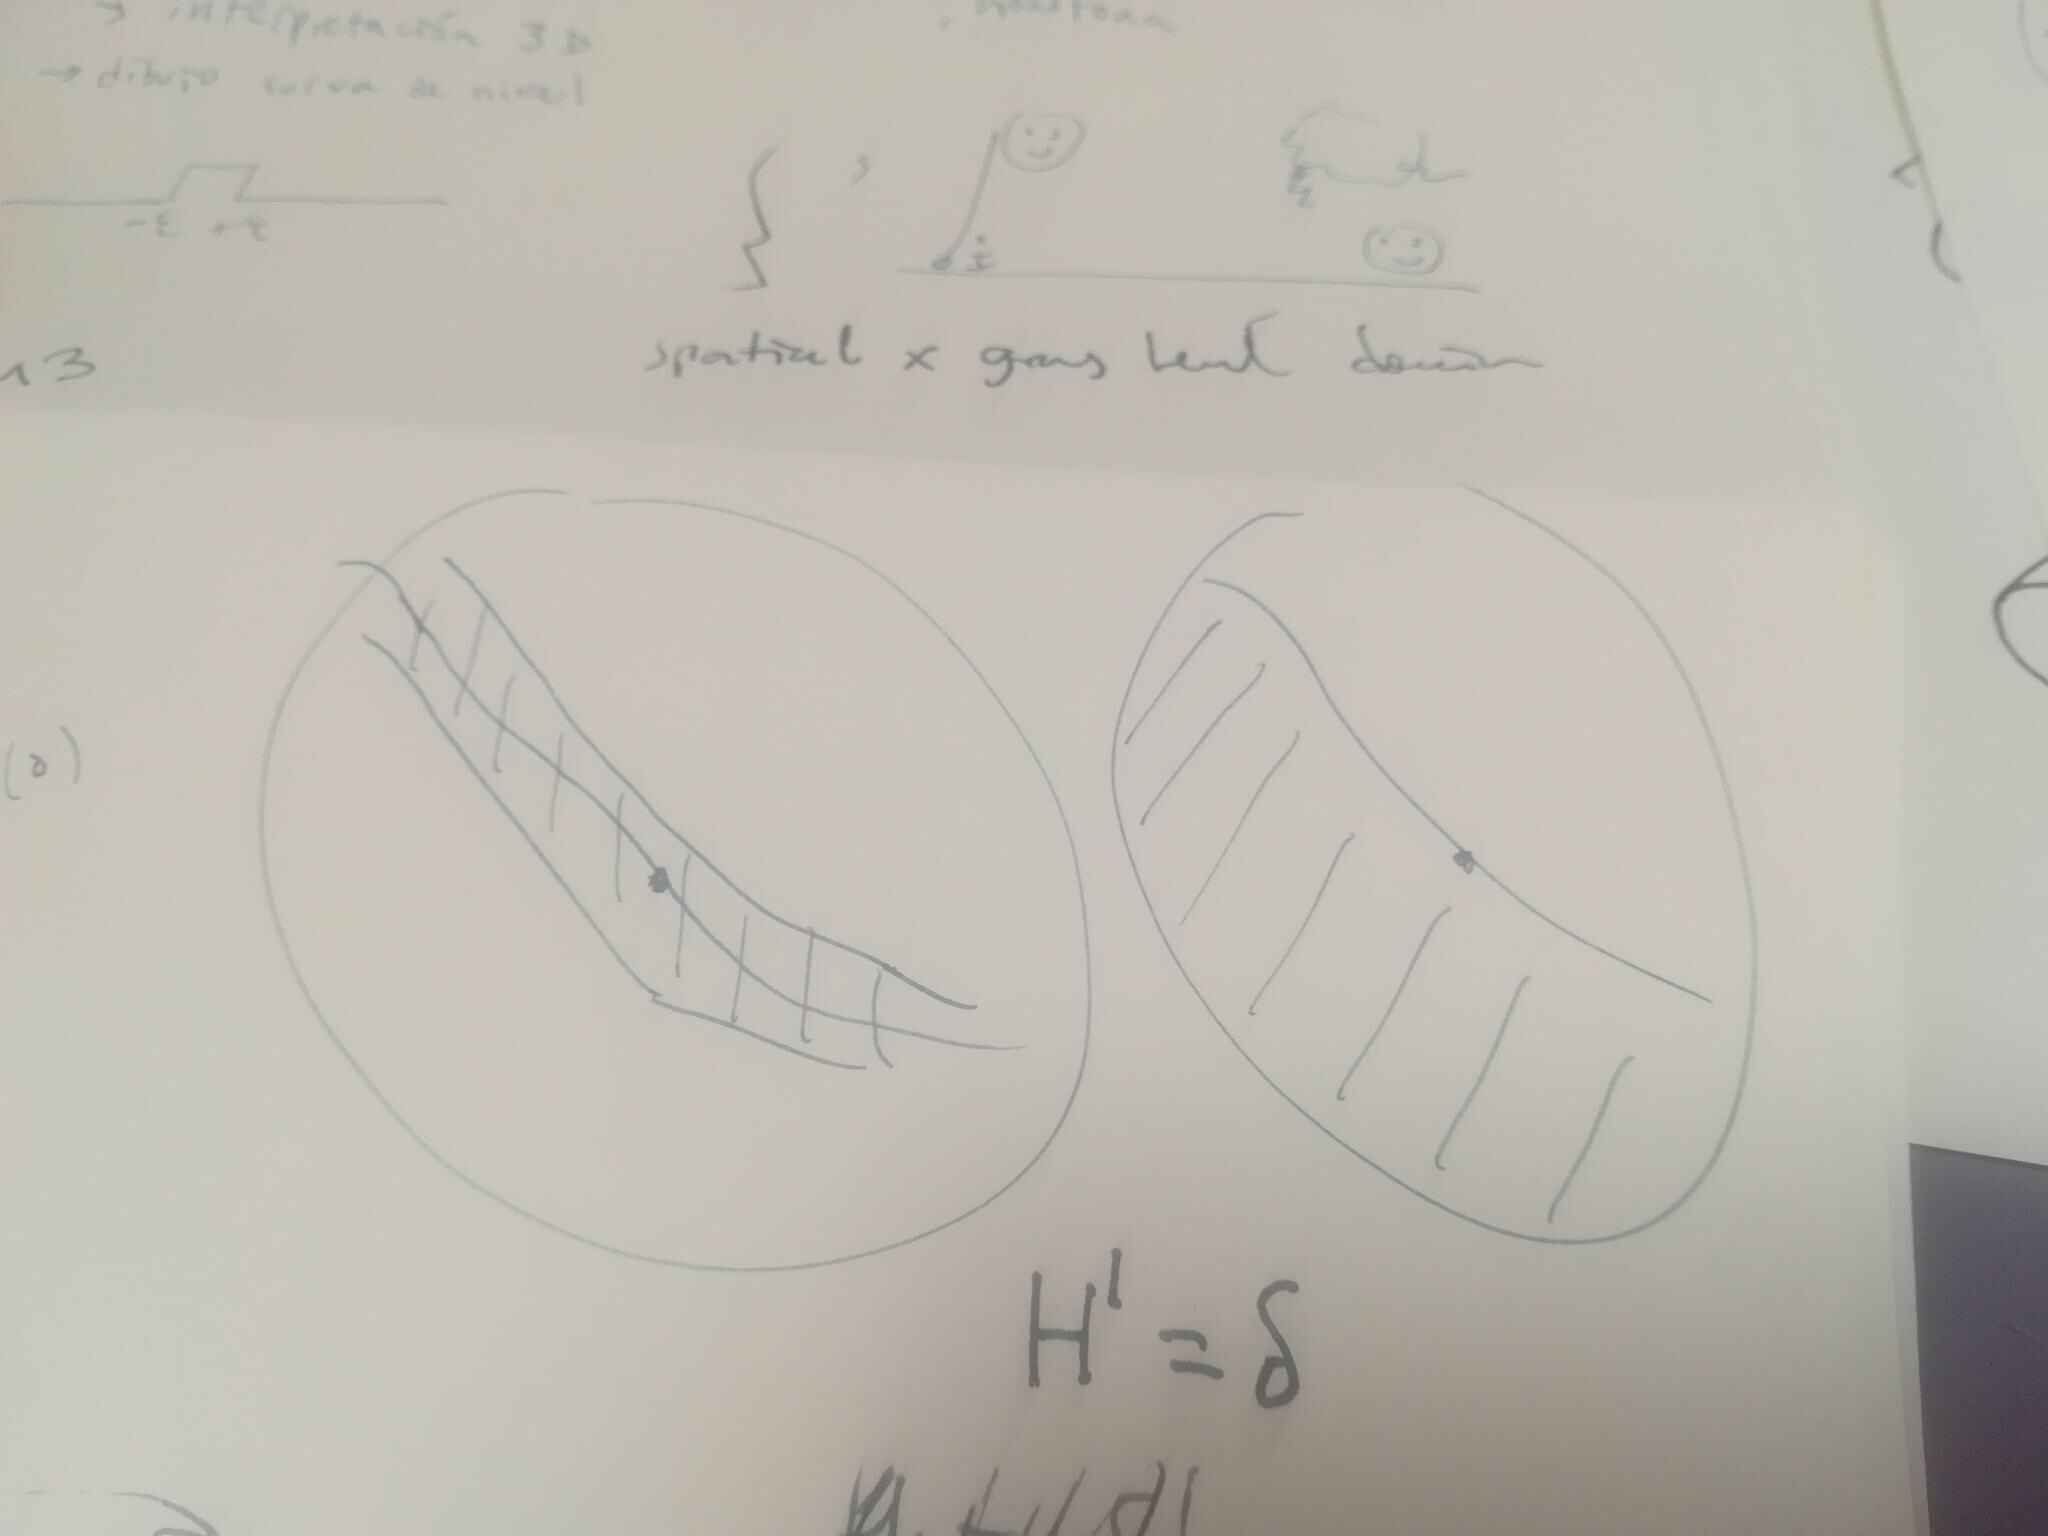
\includegraphics[width=0.7\linewidth]{f/bilateral-vs-krt.jpg}
	\end{center}
	\caption{\label{fig:bilateral-vs-krt}
	Bilateral filter domain vs KRT domain.
	}
\end{figure}

Using a similar notation as in our work, the bilateral
filter~\cite{tomasi1998bilateral,durand2002fast,paris2009bilateral} is defined
as
\begin{equation}\label{eq:bilateral}
\textsc{bil}_{\kappa,f}(u)(x) =
\frac{\int u(y) \kappa(y-x) f\big(u(y)-u(x)\big) \mathrm{d} y}
     {\int \kappa(y-x) f\big(u(y)-u(x)\big) \mathrm{d} y}
\end{equation}
where $\kappa$ is a spatial kernel and $f$ is a similarity function used to
compare image gray levels.  In a typical case, both $\kappa$ and $f$ are
Gaussian centered in zero.

The are two particular cases of this filter that justifies its name.  First,
when $f=1$, the result is the convolution of $u$ by $\kappa$, i.e. a local mean
weighted by the kernel.  Second, when $\kappa=1$ the range filter is obtained,
which produce a mean of similar gray levels globally allover the image.  The
two operations combined produces a local mean of gray-levels.

Formally, the denominator of Eq.~\ref{eq:bilateral} is similar to the kernel
rank transform (with some minor differences in the order of the indexes) with
the comparison function $\sigma$ replaced by the similarity function $f$.
The difference in name is reflected in its definition and use.  The similarity
function $f$ is typically symmetric with a maximal in zero, and going to
zero at plus and minus infinity.  On the other hand, the comparison function
$\sigma$ is typically monotonically increasing.  In both cases, the filtering
can be interpreted as as 3D filtering in the spatial-gray-level domain (see
section~\ref{sec:X}).

Conceptually, the bilateral filter is a weighted local mean of the image in a
domain defined as in figure~\ref{fig:bilateral-vs-krt}(left); the kernel rank
transform is given by the integral of the kernel in a domain defined as in
figure~\ref{fig:bilateral-vs-krt}(right).  In both cases the domain is defined
by the level-line of the point, but in former case it is narrow region around
the level-line (the points which have a \emph{similar} gray-level) while in the
latter the domain it is the lower-level set.


\subsection{Limit for a constant kernel}

In the limit when~$\kappa$ is constant, the rank transform is the histogram
equalization of~$u$.  To see this, notice that the function
\[
H(\lambda) = \int\mathbf{1}_{[u\ge\lambda]}
\]
is the (reverse) accumulated histogram of~$u$.  This is, the area of the domain
where~$u$ has a value larger than~$\lambda$.  The derivative of~$H$ is thus the
histogram of~$u$.

Notice that this global/local relation is the same as found in local
histogram normalization techniques.
The following two formulations are really similar:

Ref. Sapiro, Caselles,  "Histogram modification via Differential Equations",
formula (21)~\cite{sapiro1997histogram}

Ref. Bertalmío et al. "evidence for the intrinsically nonlinear nature of
receptive fields in vision", formula (10) and next~\cite{bertalmio2020evidence}


\subsection{Bilateral interpretation}

NOTE: the piece of text below concerns the justification of the krt
definition.  It may be removed 

The accumulated histogram can be ``smoothed'' by using a smooth sigmoid instead
of the discontinuous indicator function.  For example, let~$\sigma$ be a step
function centered at~$0$, we can define the~$\sigma$-smoothed accumulated
histogram of~$u$ by
\[
H_\sigma(\lambda)=\int\sigma(u(x)-\lambda)\mathrm{d}x
\]
Thus, a more general version of the definition for the rank transform is
\begin{equation}\label{eq:generalrank}
	\textsc{krt}_{\kappa,\sigma}(u)(x)=\int \kappa(x-y)\sigma(u(x)-u(y))\mathrm{d}y
\end{equation}
in the limit when~$\sigma$ is the heaviside step function we recover the
original definition~$\textsc{krt}_\sigma(u)$.

Notice that the convolution formalism given in
equation~(\ref{eq:convolution1}) puts the~$\sigma$ and~$\kappa$ smoothings
on an equal footing.  Indeed, by defining
\[
	K_\sigma(x,t)=\kappa(x)\sigma'(t)
\]
we can write formula~(\ref{eq:generalrank}) as
\begin{equation}\label{eq:convolution2}
	\textsc{krt}_{\kappa,\sigma}(u)(x)=(U*K_\sigma)(x,u(x)).
\end{equation}

%SCRIPT gnuplot > f/plot_heavisides.png <<EOF
%SCRIPT set term pngcairo size 500,400
%SCRIPT gap(x)=x>1?1:(x<-1?0:(0.5*(x+1)))
%SCRIPT plot [-1.5:1.5] [-0.25:1.75] 0.5+atan(x*pi)/pi,1/(1+exp(-4*x)),gap(2*x),0.5+erf(x*sqrt(pi))/2
%SCRIPT EOF

\begin{figure}
	\centering
	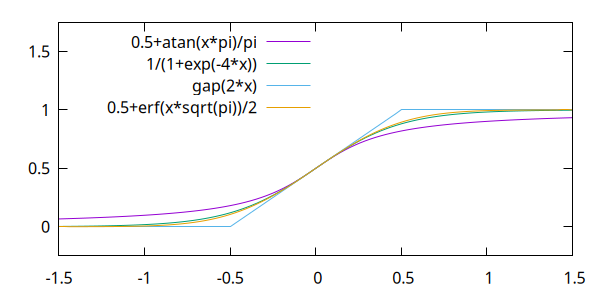
\includegraphics[width=0.5\linewidth]{f/plot_heavisides.png}
	\caption{Plots of the ``smooth heavisides''~$\sigma$ implemented in
	our program.  In all cases the parameter is set to~$1$, which
	corresponds to a slope of~$1$ at the origin.}
	\label{fig:heavisides}
\end{figure}



\section{Implementation}

The implementation of the kernel rank transform is almost a straightforward
adaptation of formula~\ref{eq:rtdef} for discrete images, with the integral
replaced by a sum.

TODO: Pseudocode of the krt algorithm.

TODO: pseudocode of a few kernels (square, normalized )

TODO: discuss a subtlety of the implementation.  For the classical case
(binary kernel and heaviside step) we want the following three conditions to
hold: (1) for constant regions the krt is exactly 0.5;  (2) at the global
maximum, the krt is exactly 1; (3) at the global minimum, the krt is exactly
0.  These conditions are satisfied by the given implementation, that omits
the central point in the sum, and in the kernel normalization.

Discrete implementation for a small support kernel, written in C

{\small
\begin{verbatim}
krt [options] KERNEL [IN [OUT]]

IN : input image (by default, stdin)
OUT : output image of the same size as the input (by default, stdout)
KERNEL : string that specifies the kernel k  Examples:

"file.npy" : the kernel is given by a numeric array, the center is at the
center of the image

"gauss:S" : the kernel is a gaussian of that sigma=S (in pixels)

"disk:R" : disk of radius R

"rectangle:N" : centered rectangle of size (2M+1)x(2M+1), where M=floor(N)

options:

-p 0 : getpixel = 0 outside the original image domain
-p 1 : getpixel = nearest neighbor
-p 2 : getpixel = symmetric extension
... (periodic, etc)

\end{verbatim}
}

Generic implementation as a 3d convolution (consider the problem of
gray-scale sampling!), written in C

{\small
\begin{verbatim}
krt3d [options] KERNEL [IN [OUT]]

IN : input image (by default, stdin)
OUT : output image of the same size as the input (by default, stdout)
KERNEL : string that specifies the kernel k  Examples:

"file.npy" : the kernel is given by a numeric array, the center is at the
center of the image, extended by zero outside of its domain

"gauss:S" : the kernel is a gaussian of that sigma=S (in pixels)

"riesz:S" : riesz kernel of parameter S

options:

-s 255 : gray-scale factor
-n 256 : number of gray-scale bins

future:
-h s : gray-level filtering parameter

\end{verbatim}
}

Verification that both implementations give the same result

Comparison of both implementations (table of running times depending on
kernel size/number of gray levels?)

\section{Examples and applications}

\subsection{Experiment: Adelson checkerboard }

% f/adelson.png
%SCRIPT ./krt square5  f/adelson.png |qauto -p 0 - f/adelson_sq5.png
%SCRIPT ./krt gauss5   f/adelson.png |qauto -p 0 - f/adelson_g5.png
%SCRIPT ./krt landc25  f/adelson.png |qauto -p 0 - f/adelson_l25.png
%SCRIPT ./krt square5 -h gap2 f/adelson.png|qauto -p 0 - f/adelson_sq5_gap2.png
%SCRIPT ./krt gauss5  -h gap2 f/adelson.png|qauto -p 0 - f/adelson_g5_gap2.png
%SCRIPT ./krt landc25 -h gap2 f/adelson.png|qauto -p 0 - f/adelson_l25_gap2.png
%SCRIPT ./krt square5 -h gap10 f/adelson.png|qauto -p 0 - f/adelson_sq5_gap10.png
%SCRIPT ./krt gauss5  -h gap10 f/adelson.png|qauto -p 0 - f/adelson_g5_gap10.png
%SCRIPT ./krt landc25 -h gap10 f/adelson.png|qauto -p 0 - f/adelson_l25_gap10.png
%SCRIPT ./krt square5 -h gap20 f/adelson.png|qauto -p 0 - f/adelson_sq5_gap20.png
%SCRIPT ./krt gauss5  -h gap20 f/adelson.png|qauto -p 0 - f/adelson_g5_gap20.png
%SCRIPT ./krt landc25 -h gap20 f/adelson.png|qauto -p 0 - f/adelson_l25_gap20.png
%SCRIPT ./krt square5 -h gap200 f/adelson.png|qauto -p 0 - f/adelson_sq5_gap200.png
%SCRIPT ./krt gauss5  -h gap200 f/adelson.png|qauto -p 0 - f/adelson_g5_gap200.png
%SCRIPT ./krt landc25 -h gap200 f/adelson.png|qauto -p 0 - f/adelson_l25_gap200.png

\begin{tabular}{cccc}
	& square 5 & gauss 5 & land25 \\
	h&
	\includegraphics[width=0.3\linewidth]{f/adelson_sq5.png} &
	\includegraphics[width=0.3\linewidth]{f/adelson_g5.png} &
	\includegraphics[width=0.3\linewidth]{f/adelson_l25.png} \\
	gap2&
	\includegraphics[width=0.3\linewidth]{f/adelson_sq5_gap2.png} &
	\includegraphics[width=0.3\linewidth]{f/adelson_g5_gap2.png} &
	\includegraphics[width=0.3\linewidth]{f/adelson_l25_gap2.png} \\
	gap10&
	\includegraphics[width=0.3\linewidth]{f/adelson_sq5_gap10.png} &
	\includegraphics[width=0.3\linewidth]{f/adelson_g5_gap10.png} &
	\includegraphics[width=0.3\linewidth]{f/adelson_l25_gap10.png} \\
	gap20&
	\includegraphics[width=0.3\linewidth]{f/adelson_sq5_gap20.png} &
	\includegraphics[width=0.3\linewidth]{f/adelson_g5_gap20.png} &
	\includegraphics[width=0.3\linewidth]{f/adelson_l25_gap20.png} \\
	gap200&
	\includegraphics[width=0.3\linewidth]{f/adelson_sq5_gap200.png} &
	\includegraphics[width=0.3\linewidth]{f/adelson_g5_gap200.png} &
	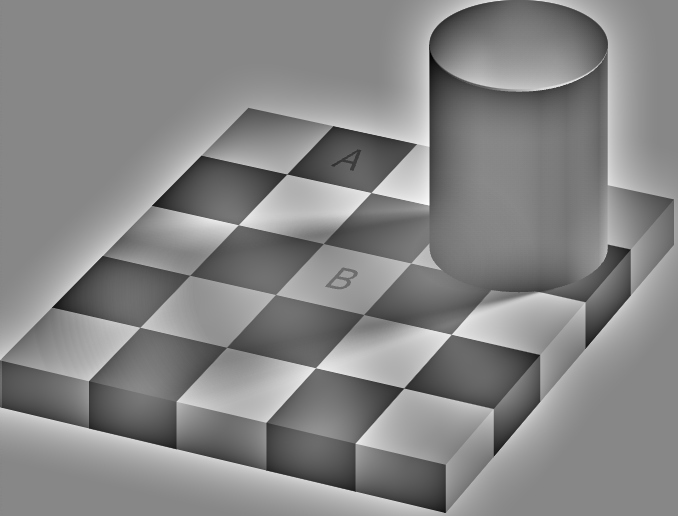
\includegraphics[width=0.3\linewidth]{f/adelson_l25_gap200.png} \\
\end{tabular}

%SCRIPT ./krt square3  f/adelson.png |qauto -p 0 - f/adelson_sq3.png
%SCRIPT ./krt square13  f/adelson.png |qauto -p 0 - f/adelson_sq13.png
%SCRIPT ./krt square33  f/adelson.png |qauto -p 0 - f/adelson_sq33.png
%SCRIPT ./krt gauss3   f/adelson.png |qauto -p 0 - f/adelson_g3.png
%SCRIPT ./krt gauss13   f/adelson.png |qauto -p 0 - f/adelson_g13.png
%SCRIPT ./krt gauss33   f/adelson.png |qauto -p 0 - f/adelson_g33.png
%SCRIPT ./krt landc3   f/adelson.png |qauto -p 0 - f/adelson_l3.png
%SCRIPT ./krt landc13   f/adelson.png |qauto -p 0 - f/adelson_l13.png
%SCRIPT ./krt landc33   f/adelson.png |qauto -p 0 - f/adelson_l33.png
\begin{tabular}{cccc}
	(heaviside)& square & gauss & land \\
	3&
	\includegraphics[width=0.3\linewidth]{f/adelson_sq3.png} &
	\includegraphics[width=0.3\linewidth]{f/adelson_g3.png} &
	\includegraphics[width=0.3\linewidth]{f/adelson_l3.png} \\
	13&
	\includegraphics[width=0.3\linewidth]{f/adelson_sq13.png} &
	\includegraphics[width=0.3\linewidth]{f/adelson_g13.png} &
	\includegraphics[width=0.3\linewidth]{f/adelson_l13.png} \\
	33&
	\includegraphics[width=0.3\linewidth]{f/adelson_sq33.png} &
	\includegraphics[width=0.3\linewidth]{f/adelson_g33.png} &
	\includegraphics[width=0.3\linewidth]{f/adelson_l33.png} \\
\end{tabular}

%SCRIPT ./krt square3  -h gap20 f/adelson.png |qauto -p 0 -  f/adelson_sq3_gap20.png
%SCRIPT ./krt square13 -h gap20  f/adelson.png |qauto -p 0 - f/adelson_sq13_gap20.png
%SCRIPT ./krt square33 -h gap20  f/adelson.png |qauto -p 0 - f/adelson_sq33_gap20.png
%SCRIPT ./krt gauss3   -h gap20 f/adelson.png |qauto -p 0 -  f/adelson_g3_gap20.png
%SCRIPT ./krt gauss13  -h gap20  f/adelson.png |qauto -p 0 - f/adelson_g13_gap20.png
%SCRIPT ./krt gauss33  -h gap20  f/adelson.png |qauto -p 0 - f/adelson_g33_gap20.png
%SCRIPT ./krt landc3   -h gap20 f/adelson.png |qauto -p 0 -  f/adelson_l3_gap20.png
%SCRIPT ./krt landc13  -h gap20  f/adelson.png |qauto -p 0 - f/adelson_l13_gap20.png
%SCRIPT ./krt landc33  -h gap20  f/adelson.png |qauto -p 0 - f/adelson_l33_gap20.png
\begin{tabular}{cccc}
	(gap20) & square & gauss  & land \\
	3&
	\includegraphics[width=0.3\linewidth]{f/adelson_sq3_gap20.png} &
	\includegraphics[width=0.3\linewidth]{f/adelson_g3_gap20.png} &
	\includegraphics[width=0.3\linewidth]{f/adelson_l3_gap20.png} \\
	13&
	\includegraphics[width=0.3\linewidth]{f/adelson_sq13_gap20.png} &
	\includegraphics[width=0.3\linewidth]{f/adelson_g13_gap20.png} &
	\includegraphics[width=0.3\linewidth]{f/adelson_l13_gap20.png} \\
	33&
	\includegraphics[width=0.3\linewidth]{f/adelson_sq33_gap20.png} &
	\includegraphics[width=0.3\linewidth]{f/adelson_g33_gap20.png} &
	\includegraphics[width=0.3\linewidth]{f/adelson_l33_gap20.png} \\
\end{tabular}

%SCRIPT ./krt square13 -h gap2 f/adelson.png |qeasy 0 1 - f/adelson_sq13_gap2.png
%SCRIPT ./krt square13 -h logistic2 f/adelson.png |qeasy 0 1 - f/adelson_sq13_logis2.png
%SCRIPT ./krt square13 -h arctan2 f/adelson.png |qeasy 0 1 - f/adelson_sq13_atan2.png
%SCRIPT ./krt square13 -h gap10 f/adelson.png |qeasy 0 1 - f/adelson_sq13_gap10.png
%SCRIPT ./krt square13 -h logistic10 f/adelson.png |qeasy 0 1 - f/adelson_sq13_logis10.png
%SCRIPT ./krt square13 -h arctan10 f/adelson.png |qeasy 0 1 - f/adelson_sq13_atan10.png
%SCRIPT ./krt square13 -h gap20 f/adelson.png |qeasy 0 1 - f/adelson_sq13_gap20.png
%SCRIPT ./krt square13 -h logistic20 f/adelson.png |qeasy 0 1 - f/adelson_sq13_logis20.png
%SCRIPT ./krt square13 -h arctan20 f/adelson.png |qeasy 0 1 - f/adelson_sq13_atan20.png
%SCRIPT ./krt square13 -h gap200 f/adelson.png |qeasy 0 1 - f/adelson_sq13_gap200.png
%SCRIPT ./krt square13 -h logistic200 f/adelson.png |qeasy 0 1 - f/adelson_sq13_logis200.png
%SCRIPT ./krt square13 -h arctan200 f/adelson.png |qeasy 0 1 - f/adelson_sq13_atan200.png
\begin{tabular}{cccc}
	(square 13) & gap & logistic & arctan \\
	gap2&
	\includegraphics[width=0.3\linewidth]{f/adelson_sq13_gap2.png} &
	\includegraphics[width=0.3\linewidth]{f/adelson_sq13_logis2.png} &
	\includegraphics[width=0.3\linewidth]{f/adelson_sq13_atan2.png} \\
	gap10&
	\includegraphics[width=0.3\linewidth]{f/adelson_sq13_gap10.png} &
	\includegraphics[width=0.3\linewidth]{f/adelson_sq13_logis10.png} &
	\includegraphics[width=0.3\linewidth]{f/adelson_sq13_atan10.png} \\
	gap20&
	\includegraphics[width=0.3\linewidth]{f/adelson_sq13_gap20.png} &
	\includegraphics[width=0.3\linewidth]{f/adelson_sq13_logis20.png} &
	\includegraphics[width=0.3\linewidth]{f/adelson_sq13_atan20.png} \\
	gap200&
	\includegraphics[width=0.3\linewidth]{f/adelson_sq13_gap200.png} &
	\includegraphics[width=0.3\linewidth]{f/adelson_sq13_logis200.png} &
	\includegraphics[width=0.3\linewidth]{f/adelson_sq13_atan200.png} \\
\end{tabular}



\subsection{Experiment: mach bands}

%SCRIPT plambda zero:500x120 ":i 50 / floor" -o f/mach.npy
%%SCRIPT plambda zero:500x120 ":i 50 / floor randg 0.01 * +" -o f/mach.npy
%%SCRIPT plambda zero:500x120 ":i 50 / floor randg 0.1 * +" -o f/mach.npy
%SCRIPT plambda f/mach.npy '7 - 14 * 127 +' -o f/mach.png

%SCRIPT export X="set term pngcairo size 500,200;unset key;unset xtics"
%SCRIPT cat f/mach.npy|(echo "$X";cline 0)|gnuplot >f/p_mach.png

%SCRIPT ./krt square21 f/mach.npy|qeasy 0 1 - f/mach_sq21.png
%SCRIPT ./krt square21 f/mach.npy|(echo "$X";cline 0)|gnuplot >f/p_mach_sq21.png

%SCRIPT ./krt gauss7 f/mach.npy|qeasy 0 1 - f/mach_g7.png
%SCRIPT ./krt gauss7 f/mach.npy|(echo "$X";cline 0)|gnuplot >f/p_mach_g7.png

%SCRIPT ./krt cauchy3 f/mach.npy|qeasy 0 1 - f/mach_c3.png
%SCRIPT ./krt cauchy3 f/mach.npy|(echo "$X";cline 0)|gnuplot >f/p_mach_c3.png

%SCRIPT ./krt landc40 f/mach.npy|qeasy 0 1 - f/mach_la.png
%SCRIPT ./krt landc40 f/mach.npy|(echo "$X";cline 0)|gnuplot >f/p_mach_la.png


%SCRIPT plambda f/mach.npy ":i 0.004 * +" -o f/umach.npy
%SCRIPT plambda f/umach.npy '7 - 14 * 127 +' -o f/umach.png
%SCRIPT cat f/umach.npy|(echo "$X";cline 0)|gnuplot >f/p_umach.png
%SCRIPT ./krt square21 f/umach.npy|qeasy 0 1 - f/umach_sq21.png
%SCRIPT ./krt square21 f/umach.npy|(echo "$X";cline 0)|gnuplot >f/p_umach_sq21.png
%SCRIPT ./krt gauss7 f/umach.npy|qeasy 0 1 - f/umach_g7.png
%SCRIPT ./krt gauss7 f/umach.npy|(echo "$X";cline 0)|gnuplot >f/p_umach_g7.png
%SCRIPT ./krt cauchy3 f/umach.npy|qeasy 0 1 - f/umach_c3.png
%SCRIPT ./krt cauchy3 f/umach.npy|(echo "$X";cline 0)|gnuplot >f/p_umach_c3.png
%SCRIPT ./krt landc40 f/umach.npy|qeasy 0 1 - f/umach_la.png
%SCRIPT ./krt landc40 f/umach.npy|(echo "$X";cline 0)|gnuplot >f/p_umach_la.png

%SCRIPT plambda f/mach.npy ":i 0.004 * -" -o f/dmach.npy
%SCRIPT plambda f/dmach.npy '7 - 14 * 127 +' -o f/dmach.png
%SCRIPT cat f/dmach.npy|(echo "$X";cline 0)|gnuplot >f/p_dmach.png
%SCRIPT ./krt square21 f/dmach.npy|qeasy 0 1 - f/dmach_sq21.png
%SCRIPT ./krt square21 f/dmach.npy|(echo "$X";cline 0)|gnuplot >f/p_dmach_sq21.png
%SCRIPT ./krt gauss7 f/dmach.npy|qeasy 0 1 - f/dmach_g7.png
%SCRIPT ./krt gauss7 f/dmach.npy|(echo "$X";cline 0)|gnuplot >f/p_dmach_g7.png
%SCRIPT ./krt cauchy3 f/dmach.npy|qeasy 0 1 - f/dmach_c3.png
%SCRIPT ./krt cauchy3 f/dmach.npy|(echo "$X";cline 0)|gnuplot >f/p_dmach_c3.png
%SCRIPT ./krt landc40 f/dmach.npy|qeasy 0 1 - f/dmach_la.png
%SCRIPT ./krt landc40 f/dmach.npy|(echo "$X";cline 0)|gnuplot >f/p_dmach_la.png

\begin{figure}
	\begin{tabular}{cc}
		\includegraphics[width=0.45\linewidth]{f/mach.png} &
		\includegraphics[width=0.45\linewidth]{f/p_mach.png} \\
		\includegraphics[width=0.45\linewidth]{f/mach_sq21.png} &
		\includegraphics[width=0.45\linewidth]{f/p_mach_sq21.png} \\
		\includegraphics[width=0.45\linewidth]{f/mach_g7.png} &
		\includegraphics[width=0.45\linewidth]{f/p_mach_g7.png} \\
		\includegraphics[width=0.45\linewidth]{f/mach_c3.png} &
		\includegraphics[width=0.45\linewidth]{f/p_mach_c3.png} \\
		\includegraphics[width=0.45\linewidth]{f/mach_la.png} &
		\includegraphics[width=0.45\linewidth]{f/p_mach_la.png} \\
	\end{tabular}
	\caption{\label{fig:machnonoise}
		Mach bands without noise, various kernels.
	}
\end{figure}

\begin{figure}
	\begin{tabular}{cc}
		\includegraphics[width=0.45\linewidth]{f/umach.png} &
		\includegraphics[width=0.45\linewidth]{f/p_umach.png} \\
		\includegraphics[width=0.45\linewidth]{f/umach_sq21.png} &
		\includegraphics[width=0.45\linewidth]{f/p_umach_sq21.png} \\
		\includegraphics[width=0.45\linewidth]{f/umach_g7.png} &
		\includegraphics[width=0.45\linewidth]{f/p_umach_g7.png} \\
		\includegraphics[width=0.45\linewidth]{f/umach_c3.png} &
		\includegraphics[width=0.45\linewidth]{f/p_umach_c3.png} \\
		\includegraphics[width=0.45\linewidth]{f/umach_la.png} &
		\includegraphics[width=0.45\linewidth]{f/p_umach_la.png} \\
	\end{tabular}
	\caption{\label{fig:machup}
		Mach bands with up-ramp, various kernels.
	}
\end{figure}

\begin{figure}
	\begin{tabular}{cc}
		\includegraphics[width=0.45\linewidth]{f/dmach.png} &
		\includegraphics[width=0.45\linewidth]{f/p_dmach.png} \\
		\includegraphics[width=0.45\linewidth]{f/dmach_sq21.png} &
		\includegraphics[width=0.45\linewidth]{f/p_dmach_sq21.png} \\
		\includegraphics[width=0.45\linewidth]{f/dmach_g7.png} &
		\includegraphics[width=0.45\linewidth]{f/p_dmach_g7.png} \\
		\includegraphics[width=0.45\linewidth]{f/dmach_c3.png} &
		\includegraphics[width=0.45\linewidth]{f/p_dmach_c3.png} \\
		\includegraphics[width=0.45\linewidth]{f/dmach_la.png} &
		\includegraphics[width=0.45\linewidth]{f/p_dmach_la.png} \\
	\end{tabular}
	\caption{\label{fig:machdown}
		Mach bands with down-ramp, various kernels.
	}
\end{figure}

TODO (points A3' and A3'' in the TODO list): add the experiments above (mach
bands), with a smooth step function.  This renders the method non-contrast
invariant, but continuous.  And maybe closer to our perception (the three
cases of mach bands look identical before and after the krt).

\subsection{Experiment: Effect of the scale parameter}

show square rank scale-space (using square of varying side)

show gaussian rank scale-space


\subsection{Experiment: Comparison of different kernels}

maybe show other kernel scalespaces ?

multi-scale kernels (e.g. riesz scale space)

non-isotropic kernels ?
(ref. hirschmuller "7x5")



\subsection{Experiment: further parameter exploration}

Pick a reference image:
perlin noise of grain s + gaussian blur of intensity r
filter this image with gaussian-gaussian krt, varying botht parameters,
observe the effects depending on whether the parameters are larger/smaller
than s/r.


\subsection{Application: local image normalization}

sub-application: adaptive thresholding
\url{https://docs.opencv.org/4.x/d7/d4d/tutorial_py_thresholding.html}

\subsection{Application: noise uniformization}

After applying the KRT, noise becomes uniform.

This is an important difference between the original discrete rank transform
and the kernel rank transform (with a non-constant kernel like the
gaussian).  Both transforms produce an image with a locally uniform
histogram, as much as they can.  But the original rank transform, by
construction, produces an image whose values are integers between 1
and~$N^2$, while the smooth kernel rank transform will give generally
different floating point numbers.  Even for kernels with small support, it
produces images whose histogram is uniform, but much more finely quantized.

%SCRIPT plambda zero:256x256 "randg" -o f/randg.npy
%SCRIPT ./krt square7 f/randg.npy |plambda "48 * 1 + round"| ghisto -p | gnuplot > f/randg_k7_h.png
%SCRIPT ./krt gauss1.5 f/randg.npy |plambda '1000 * round 1000 /'| ghisto -p | gnuplot > f/randg_g15_h.png
\begin{figure}[p]
	\begin{tabular}{cc}
		\includegraphics[width=0.49\linewidth]{f/randg_k7_h.png} &
		\includegraphics[width=0.49\linewidth]{f/randg_g15_h.png} \\
		rank transform~$7x7$ &
		KRT~$\sigma=1.5$
	\end{tabular}
	\caption{\label{fig:histograms}
	Histograms of white Gaussian noise uniformized with a classical
	rank transform of size~$7x7$ and a kernel rank transform with a
	Gaussian of~$\sigma=1.5$ (with the same $7\times7$ support).
	}
\end{figure}


\subsection{Application: image comparison}

If we have images of the same scene with very different dynamic ranges, the
rank transform allows to compare them directly.   


\section{References}

\bibliographystyle{plain}
\bibliography{refs}



\clearpage

\section*{Appendix: one-parameter operators}

We consider one-parameter families of operators~$T_s$ acting upon
functions~$u:\mathbf{R}^2\to\mathbf{R}$ of whatever regularity is required
for the definitions to make sense.  The operators do not necessarily satisfy
a semigroup property (thus $T_aT_b$ is not necessarily of the form~$T_c$ for
any~$c$), and they are not necessarily the identity for~$s=0$.

\begin{tabular}{l|l|l}
	name & $T_s(u)(x)$ & $T_0(u)(x)+A[u]s+\cdots$ \\
	\hline
	heat &
	$\displaystyle G_s*u$ &
	$\displaystyle u-\Delta u\frac{s^2}2+O(s^3)$ \\
	reverse heat &
	$\displaystyle (G_s^{-1}*u)(x)$ &
	$\displaystyle u(x)+\Delta u(x)\frac{s^2}2+O(s^3)$ \\
	$a$-shift &
	$\displaystyle u(x-sa)$ &
	$\displaystyle u(x)-a\cdot\nabla u(x) s +O(s^2)$ \\
	dilation &
	$\displaystyle \sup_{y\in B_s(x)}u(y)$ &
	$\displaystyle u(x)+\left\|\nabla u(x)\right\| s +O(s^2)$ \\
	erosion &
	$\displaystyle \inf_{y\in B_s(x)}u(y)$ &
	$\displaystyle u(x)-\left\|\nabla u(x)\right\| s +O(s^2)$ \\
	median &
	$\displaystyle \mathrm{med}_{y\in B_s(x)}u(y)$ &
	$\displaystyle u(x)-\left\|\nabla u(x)\right\|\mathrm{div}\left(
	\frac{\nabla u(x)}{\left\|\nabla u(x)\right\|}
	\right)s +O(s^2)$ \\
	rof &
	$\displaystyle \arg\min_{v}\left\{\int\left\|\nabla
	v\right\|+\frac1{2s}\int(u-v)^2\right\}$ &
	$\displaystyle u(x)-\mathrm{div}\left(
	\frac{\nabla u(x)}{\left\|\nabla u(x)\right\|}
	\right)s +O(s^2)$ \\
	krt &
	$\displaystyle \int G_s(x-y)H(u(x)-u(y))\mathrm{d}y$ &
	$\frac12+\mathrm{div}\left(
	\frac{\nabla u(x)}{\left\|\nabla u(x)\right\|}
	\right)s +O(s^2)$ \\
	fraclap &
	$\displaystyle \mathcal{F}^{-1}(e^{-s|\xi|^\alpha}\hat u(\xi))$ &
	$\displaystyle u(x)-(-\Delta)^{-\alpha/2}u(x)s+O(s^2)$ \\
	riesz &
	$\displaystyle (-\Delta)^{-s/2}u(x)$ &
	$\displaystyle u+sA[u]+O(s^2)$\\
	& & $\qquad A[u] = -\mathcal{F}^{-1}(\log|\xi|\hat u(\xi))$
\end{tabular}
% Copy-paste from chatgpt below (notice that the reference by Cucker-Smale
% is completely hallucinated!  upon further request it even gave a doi,
% which turned out to be non-existent)
%
% For infinitesimal generators of morphological operators and nonlinear
% shift-invariant evolutions, see:
%
% G. Aubert and P. Kornprobst, Mathematical Problems in Image Processing,
% Springer, 2006 — detailed treatment of nonlinear PDEs, morphological
% evolutions, and their generators.
%
% J.-M. Morel and S. Solimini, Variational Methods in Image Segmentation,
% Birkhäuser, 1995 — includes curvature motion and related operators.
%
% J. Serra, Image Analysis and Mathematical Morphology, Academic Press, 1982 —
% foundational on morphological operators.
%
% F. Cucker and S. Smale, "On the Mathematical Foundations of Morphological
% Image Processing," Journal of Mathematical Imaging and Vision, 2002 —
% discusses infinitesimal generators in morphology.
%
% L. Ambrosio, N. Gigli, and G. Savaré, Gradient Flows in Metric Spaces and in
% the Space of Probability Measures, Birkhäuser, 2008 — general theory of
% nonlinear semigroups relevant to total variation flow.
%
% For fractional and pseudodifferential operators with logarithmic symbols:
%
% L. Hörmander, The Analysis of Linear Partial Differential Operators, Vol.
% III, Springer, 1985 — theory of pseudodifferential operators.
%
% E. M. Stein, Singular Integrals and Differentiability Properties of
% Functions, Princeton University Press, 1970.
%
% These provide rigorous frameworks for generators beyond classical linear
% semigroups.

In the ideal case, we have a one-parameter semigroup of operators~$T_s$,
defined for~$s\ge 0$ over functions~$u:\mathbf{R}^2\to\mathbf{R}$.
This family of operators is such that~$T_0$ is the identity (or, at
least tends to the identity as~$s\to 0^+$) and satisfy the semigroup
property~$T_rT_s=T_{r+s}$.  In that case, we can define the infinitesimal
generator of~$T$ as the operator
\[
	Au = \lim_{s\to0}\frac{T_su-u}s
\]
and then we can write the asymptotic expansion of~$T_s$
\[
	T_su = u + sAu + \frac{s^2}2 A^2u + \frac{s^3}6 A^3u+\cdots
\]

Notice that the family~$T_s$ can be recovered from its infinitesimal
generator~$A$ by means of the exponential:
\[
	T_su := e^{sA}u
	\equiv
	\lim_{n\to\infty}\left(I+\frac1nA\right)^nu
	\equiv
	\lim_{N\to\infty}\sum_{n=0}^N \frac{s^n}{n!}A^nu
\]
This allows to build a one-parameter semigroup from a single, moderately
well-behaved, operator~$A$.

Another way to recover~$T_s$ from~$A$ is by solving the following PDE
for~$v(t,x)$
\[
	\begin{cases}
		v_t = Av  \\
		v(0,x)=u(x)
	\end{cases}
\]
and then set~$T_s(u)(x)=v(s,x)$.

The canonical example of all of this is the translation-semigroup of a
constant
speed~$a\in\mathbf{R}^2$.  We have~$T_su(x)=u(x-sa)$, whose infinitessimal
generator is~$Au=a\cdot\nabla u$ and satisfies the linear transport
equation~$u_t=a\cdot\nabla u$.

Another famous example is the heat semigroup~$T_su=G_{s^2} * u$
where~$G_{s^2}$ is the gaussian kernel of size~$s$ (maybe missing a constant
2 somewhere...).  The infinitesimal generator is the laplacian and it
satisfies the heat equation.

A simple variation of the heat semigroup:  anisotropic
diffusion~$u_t=\mathrm{div}\left(D\nabla u\right)$ where~$D$ is a (possibly
position-varying) diffusion matrix.  The PDE and infinitesimal generator are
just as clear as for the Gaussian case, but here the semigroup~$T_s$ does not
admit a closed-form solution when~$D$ is not constant.

If~$T_s$ is shift-covariant and linear then it is given by some fourier
multiplier~$T_su=\mathcal{F}^{-1}(m(s,\xi)\hat{u}(\xi))$.  In that case~$Au$
is not necessarily a differential operator on~$u$, but a more general
pseudo-differential operator.

\bigskip

When~$T_s$ is not a semigroup, some of the constructions above break down,
but not all.  For example, we can still write the Taylor development
\[
	T_su = A_0u + A_1us+A_2u\frac{s^2}2+A_3u\frac{s^3}{3!}+\cdots
\]
but the operators~$A_i$ are in general unrelated, and not powers of a single
operator operator~$A$.

An easy example of that is to take some operator~$A$ and
define~$T_su=u+sAu$.  This is not a semigroup, but still you can say that
its ``first order generator'' is~$A$.  Obviously these construcitons are not
unique: there will be many one-parmeter families of operators whose
first-order generator is~$A$, for example~$T_su=\frac{1}{1-sAu}$ and so on.
Among all of these, there is a particularly interesting one, which is the
semigroup~$T_su=e^{sA}u$.

The act of building a semigroup from a non-semigroup~$T_s$, by
taking~$e^{sA}$ where~$A$ is the first-order generator of~$T$ is apparently
called the Moreau-Yosida projection.

Tentative: the krt does not define a semigroup, but the coresponding
semigroup is the solutions of the backward mean curvature motion, or perona
malik-equation.  This is associated to iterated median filters, which are
known not to approximate the corresponding pde.







\end{document}


% vim:set tw=76 filetype=tex spell spelllang=en ts=2 sw=2:
